\chapter{Crosstalk Cancellation}
\label{chap:crosstalk}
\thispagestyle{fancy}

Crosstalk poses a significant challenge to the development of large quantum information processing architectures.
Among the various forms of crosstalk, such as signal crosstalk \cite{signal_crosstalk}, measurement crosstalk \cite{meas_crosstalk} or quantum-mechanical crosstalk \cite{QM_crosstalk}, microwave signal crosstalk is generally more problematic for superconducting qubits.

In this chapter, we demonstrate crosstalk cancellation in our setup. 
We employ a method similar to the one described in Nuerbolati \emph{et al.} \cite{crosstalk}.

\section{Introduction}

\emph{Microwave signal crosstalk} in superconducting qubits refers to the unwanted interaction between a qubit and microwave signals intended for different qubits or components within the circuit.
Microwave signal crosstalk can lead to errors in quantum operations and measurements.
Therefore, mitigating or eliminating crosstalk is essential for ensuring the proper functioning of superconducting qubit devices.

We study the problem using the two storage qubits on our device, where the dedicated charge lines may couple to the other qubit.
In particular, we differentiate between the two qubits by labeling them as either the \emph{control} qubit, driven by the microwave signal, or the \emph{target} qubit, influenced by the control drive due to crosstalk.
The control qubit's frequency in our setup is $\omega_c = \SI{6.0217}{\giga \hertz}$, while the target's frequency is $\omega_t = \SI{6.0286}{\giga \hertz}$.
They are detuned by less then $\SI{10}{\mega \hertz}$.

\begin{comment}
We consider the effect of the control drive on the target qubit and the target qubit as frequency shift given by alternative-current (AC) Stark effect \cite{AC_starl}.
The off-resonant control drive induces a frequency shift on the control qubit given by
\begin{equation}
\label{eq:stark_ac}
    \ac (\Omega, \Delta) = 
    \text{sgn} (\Delta) ( \sqrt{\Omega^2 + \Delta^2} - |\Delta|) ,
    %\simeq \frac{\Omega^2}{2 \Delta} ,
\end{equation}
where $\Delta = \omega_t - \omega_c$ is the detuning between the two qubits and $\Omega$ is the Rabi frequency of the crosstalk drive if it is on resonance with the target qubit.
%The approximation of \cref{eq:stark_ac} is justified when $\Omega \ll |\Delta|$.
This frequency shift effectively changes the operating frequency of the target qubit and it is therefore a source of gate error.

The crosstalk signal can be cancelled by interfering it with a  compensation pulse with same shape, frequency and amplitude but shifted by  $180^\circ $ out of phase.
This compensation signal has to be calibrated using the target qubit as probe, since the effective amplitude and phase of the control signal when it reaches the target qubit is unknown.

Figure~\ref{fig:detunings} highlights a significant challenge when employing long signals on the control charge line in Rabi experiments: minimal population changes are observed on the target qubit, rendering characterization difficult.
Alternatively, measuring crosstalk through induced AC Stark shift using Ramsey measurements offers a more adaptable approach.
This method allows for effective characterization even with long signals, providing greater flexibility in experimental analysis.
For this reason, we decided to assess the impact of the control drive on the target qubit by conducting Ramsey experiments, by measuring the induced AC stark shift on the target qubit.
\end{comment}

\section{Detecting Crosstalk with Rabi Measurements}

\begin{figure}[t!]
    \centering
    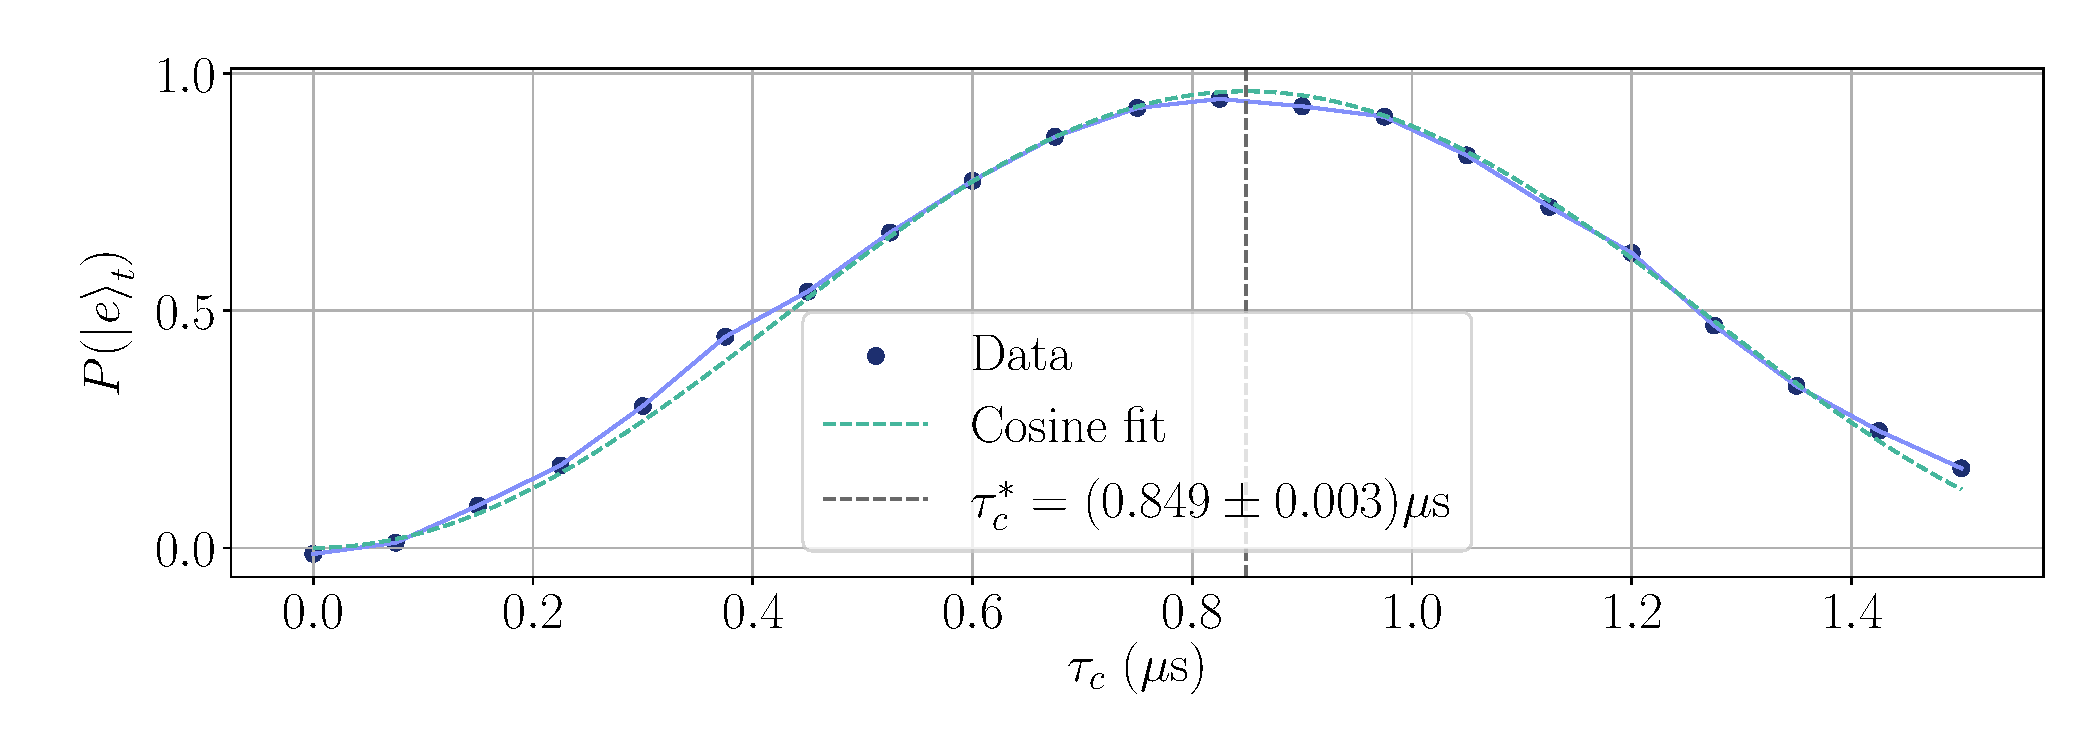
\includegraphics[width = 0.8 \textwidth]{Images/Chap2.0/sigma.pdf}
    \vspace{-0.4cm}
    \caption{Population of the excited state of the target qubit when driven by an on-resonance drive signal on the control qubit's gate line, as a function of the drive signal's duration $\tau_c$.}
    \label{fig:sigmas}
\end{figure}

We start our investigation by detecting and confirming the presence of microwave signal crosstalk, while also trying to estimate it.
As depicted in \cref{fig:sigmas}, we observe the excitation of the target qubit through the control drive, particularly when driven at resonance with the frequency of the target qubit and with the same amplitude as a standard $\pi$-rotation gate implemented on the target qubit.
The dataset has been fitted to a cosine function to obtain an approximation of the duration of the signal in order to implement a $\pi$-rotation on the target.
The calculated duration is $\tau_c^* = (0.849 \pm 0.003) \mu \text{s}$.
Dividing the standard gate time of a $\pi$-pulse driven directly on resonance on the target qubit by the estimate obtained, we deduce an approximation of the crosstalk $\xtalk$ between the gate line of the control qubit and the target qubit:
\begin{equation}
\xtalk = \frac{\SI{30}{ns}}{\tau_c^*} = (3.53 \pm 0.01) \% .
\end{equation}

\begin{figure}
    \centering
    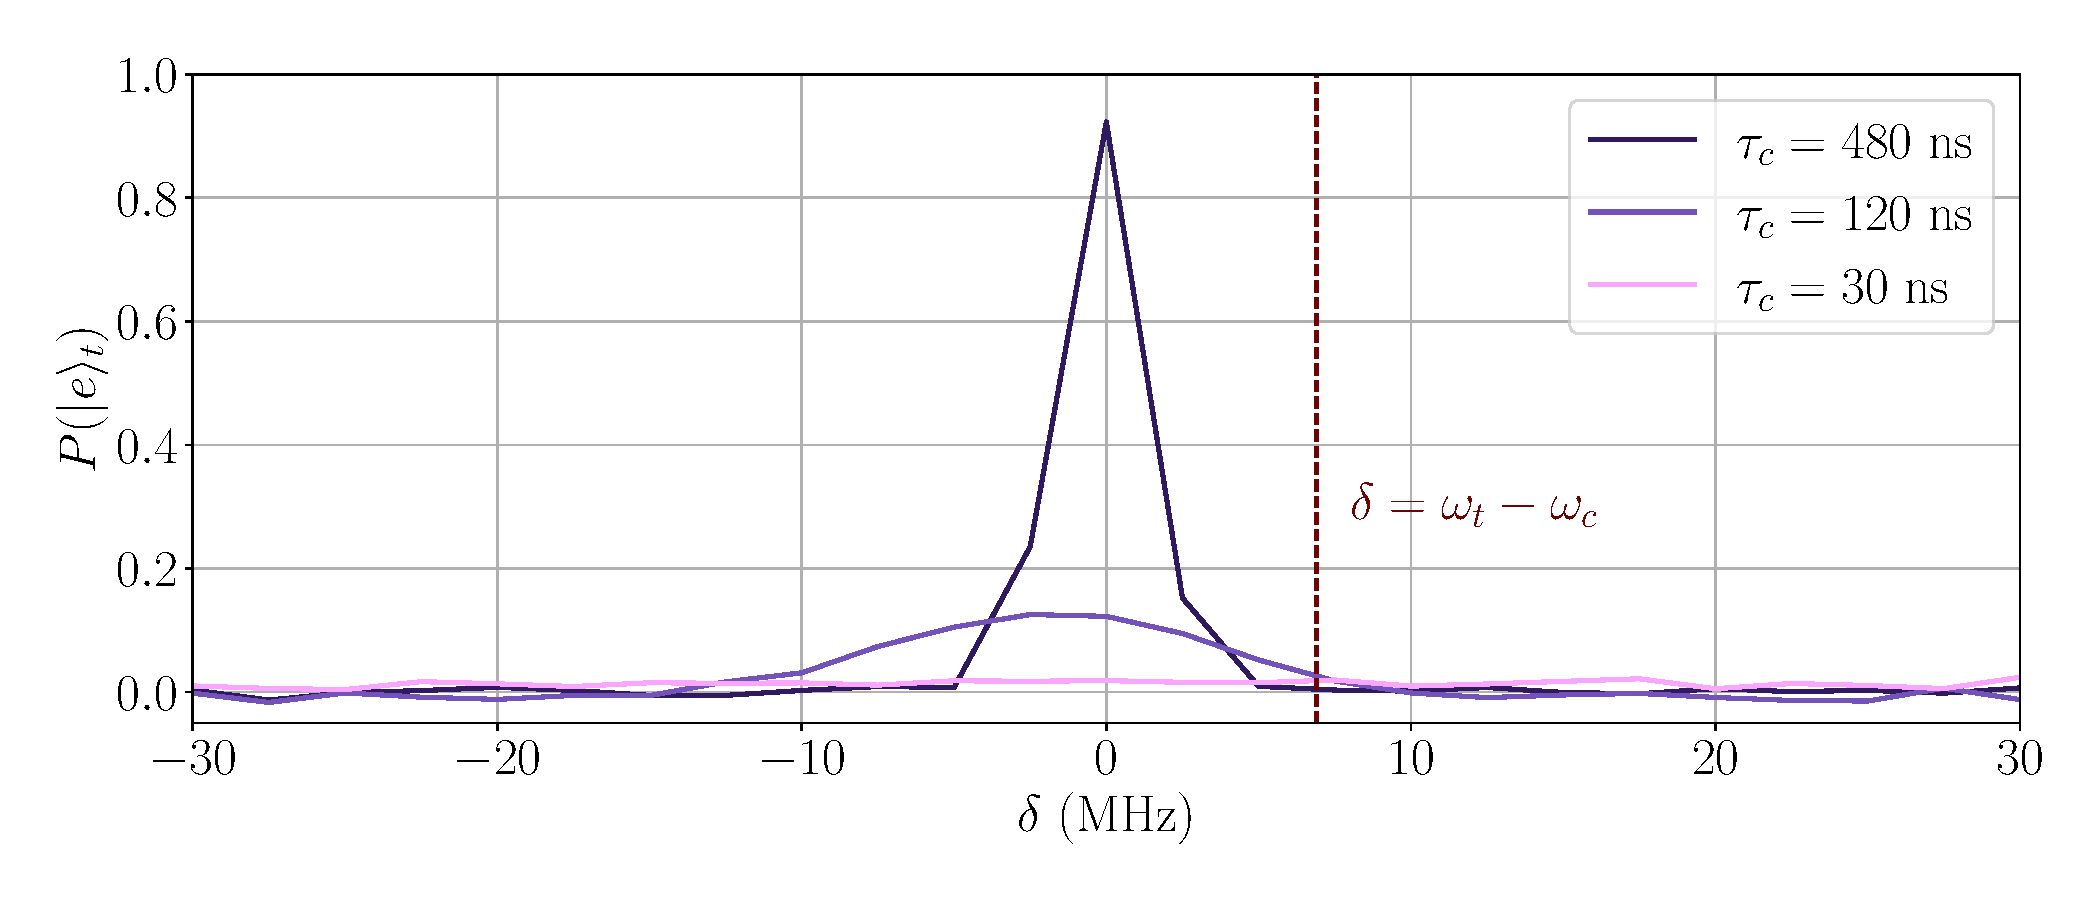
\includegraphics[width=0.8\textwidth]{Images//Chap2.0/detunings.pdf}
    \caption{Population of the excited state of the target qubit when driven through the control qubit's gate line, as a function of the detuning between the target qubit and the control drive. Results for three different values of the duration of the Gaussian-shaped signal are shown. Vertical line depicts the operational detuning between the two qubits.}
    \label{fig:detunings}
\end{figure}

We also examined the variation in the population of the target qubit with respect to the detuning $\delta$ between the target qubit's frequency and the control drive, across different values of $\tau_c$ for the Gaussian-shaped signal. 
The outcomes are depicted in \cref{fig:detunings}.
Notably, for $\tau_c = \SI{480}{ns}$, when the drive signal resonates with the target frequency, significant excitation of the qubit is observed.
Conversely, for smaller values of the duration, the peak is lower yet broader, indicating that a wider range of pulse frequencies can drive the qubit off-resonantly.
Vertical line represents the detuning between the two qubits when they are on the operational frequencies.
This represents the detuning between the target qubit and the control drive during the implementation of a standard protocol, wherein the control qubit is driven by a resonant pulse.

This outcome indicates that in our current setup, microwave signal crosstalk is hard to detect directly through Rabi type measurement.
%This observation holds true even when implementing standard operations such as a $\pi$-pulse on the control qubit, where $\sigma = \SI{5}{ns}$. 
In particular, \cref{fig:detunings} highlights that when employing long signals on the control charge line in Rabi experiments, minimal population changes are observed on the target qubit, rendering characterization difficult.
As an alternative, we can instead measure induced \emph{AC Stark effect} \cite{AC_starl} through Ramsey measurements.

In the following sections, we first review the method and present our results replicating the work introduced in Nuerbolati \emph{et al.} \cite{crosstalk}.
Next, we discuss a variant of the protocol introduced, where pulse shapes more relevant to single qubit control is used. 


%Consequently, to effectively demonstrate and subsequently cancel this crosstalk phenomenon using our method, we may need to employ techniques to amplify its effect.

\section{Measuring Crosstalk with AC Stark shift}

As already introduced in the previous section, to characterize and verify the successful cancellation of crosstalk in our device, we measure its effect as induced AC Stark shift on the target qubit.
The off-resonant control drive induces a frequency shift given by
\begin{equation}
\label{eq:stark_ac}
    \ac (\Omega, \Delta) = 
    \text{sgn} (\Delta) ( \sqrt{\Omega^2 + \Delta^2} - |\Delta|) ,
    %\simeq \frac{\Omega^2}{2 \Delta} ,
\end{equation}
where $\Delta = \omega_t - \omega_c$ is the detuning between the two qubits and $\Omega$ is the Rabi frequency of the crosstalk drive if it is on resonance with the target qubit.
%The approximation of \cref{eq:stark_ac} is justified when $\Omega \ll |\Delta|$.
This frequency shift effectively changes the operating frequency of the target qubit and it is therefore a source of gate error.

%--------------------------------------------------------------------------------------------------------------------------------------------------------------------------------------------------------------------------------------------------------------------------------------------------------------------------------------------------------------

\subsection{Measurement Protocol}

To characterize the crosstalk we implement the gate sequence depicted in \cref{fig:pulse_train_flattop}.
We run a Ramsey sequence on the target qubit, therefore the initial and the final gates executed are $\pi/2$-gates.
Subsequently, we drive the control qubit with a flat-top signal, resonant with its frequency, for a duration of $\SI{2}{\micro \second}$.
This signal can be characterized simply as a cosine pulse, defined by its amplitude $A$ and phase $\phi$.
Following a delay time $\tau_d$, we drive the target qubit with the same signal, although sweeping the relative amplitude $r$ and phase $\Delta \phi$ with respect to the control drive. 
Details on how to determine the delay time will be explained later on in \cref{sec:gaussian_shaped}.

Our goal is to identify the optimal parameters $\Vec{r} = r e^{i\Delta \phi}$ such that the compensation signal, with amplitude $rA$, phase $\phi + \Delta \phi$ and frequency $\omega_c$ effectively cancels the influence of the control drive.

\begin{figure}
    \centering
    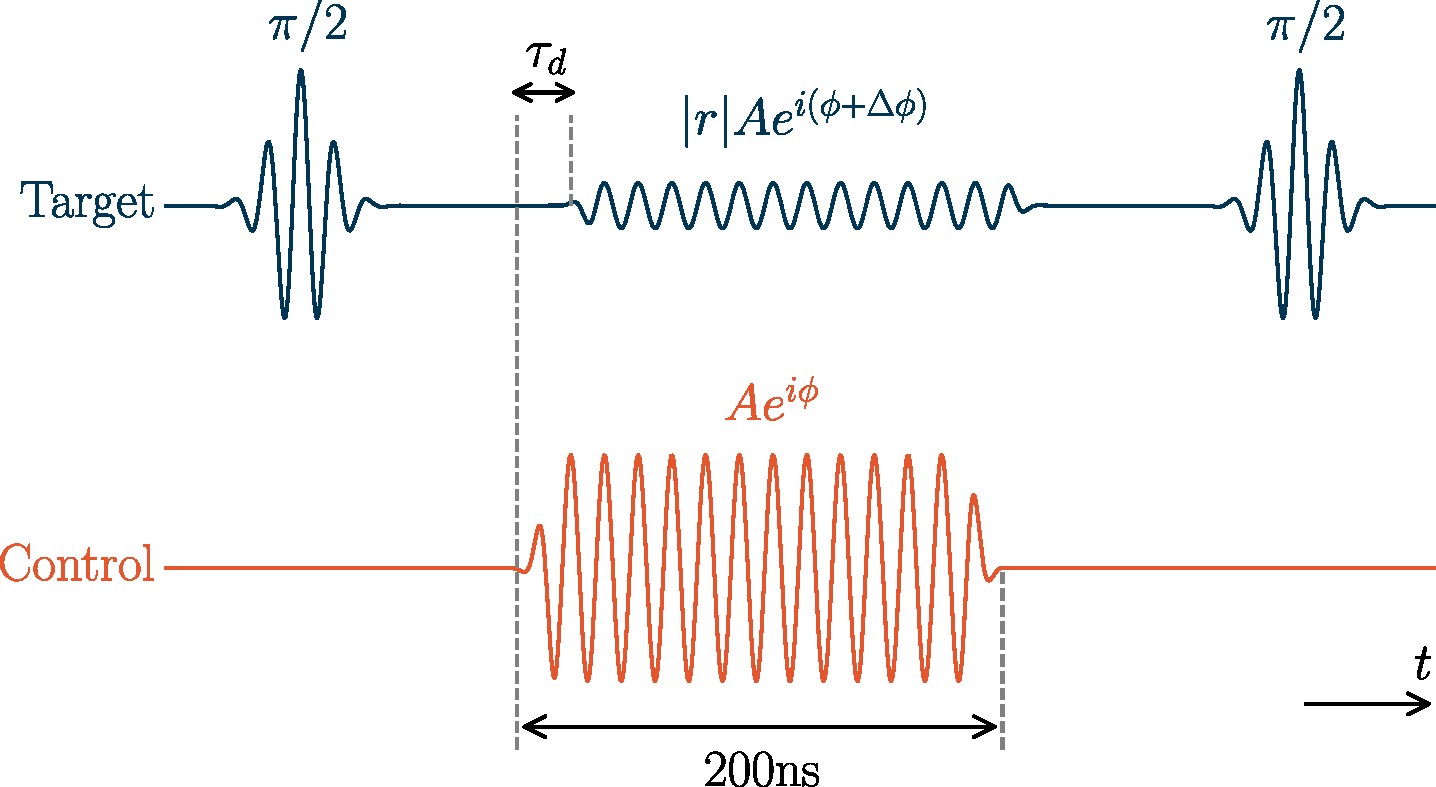
\includegraphics[width=0.85\textwidth]{Images//Chap2.0/diagram_falttop.pdf}
    \vspace{-0.5cm}
    \caption{Pulse sequence for crosstalk characterization with flat-top pulses}
    \label{fig:pulse_train_flattop}
\end{figure}

\subsection{Measurement Results}

\begin{figure}
    \centering
    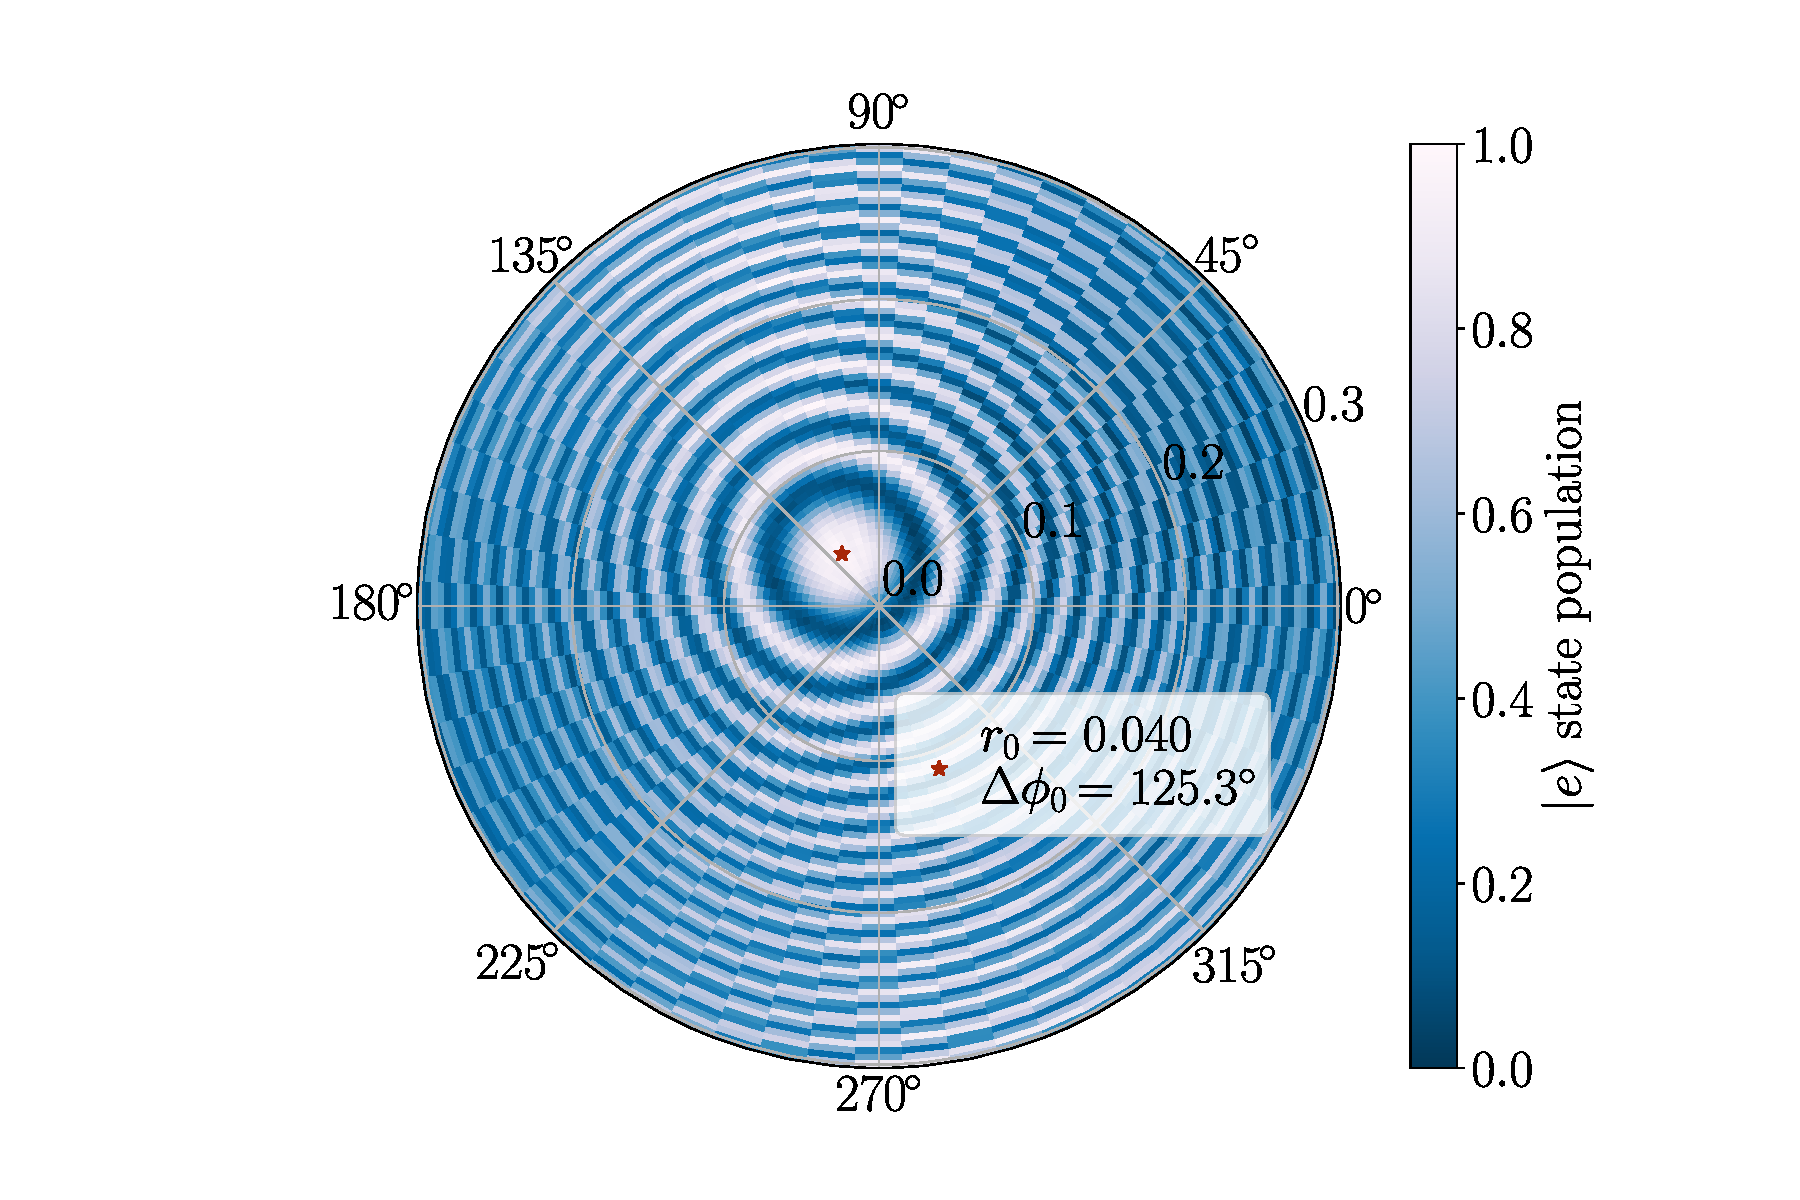
\includegraphics[width=0.9\linewidth]{Images//Chap2.0/circles.pdf}
    \vspace{-0.8cm}
    \caption{Data acquired from measurement of target qubit after gate sequence of \cref{fig:pulse_train_flattop}. Red star denotes the optimal parameters to contrast the crosstalk}
    \label{fig:circles_flat}
\end{figure}

\begin{comment}
Figure \ref{fig:circles_flat} shows the data collected from measuring the excited state population of the target qubit following the previously described pulse sequence.
Notably, the pattern observed in \cref{fig:circles_flat} resembles Newton's rings \cite{newton}.
The central point of these rings, marked by a red star, represents the optimal operational point for compensation.
As one moves outward from the center, each ring accumulates an additional $2 \pi$ phase.

The pattern is mathematically described by the equation \cite{crosstalk}:
\begin{equation}
S = \frac{1}{2}[1 + \cos\left( \ac (|\Vec{r} + \Vec{r}^*| A, \Delta) \cdot \tau \right)] ,
\end{equation}
where $S$ represents the normalized signal, $\Delta$ denotes the detuning between the qubits, and $\tau = \SI{200}{ns}$.

The central point was determined based on its symmetry.
We assessed the symmetry of the data around various points and selected the one exhibiting the most central symmetry as the center of the rings.
In this case, the cancellation parameters has been found to be $r = 0.040$ and $\phi = 125.3^\circ$.
\end{comment}

\begin{comment}
We replicate the procedure to characterize the crosstalk presented in \cite{crosstalk} and demonstrate its successful cancellation by employing the $180^\circ$ out-of-phase pulse in two scenarios:
\begin{itemize}[itemsep=3pt]
    \item \textbf{Flat-top pulses:} Initially, we drive the control qubit using $\SI{2}{\micro \second}$-long cosine-wave pulses, replicating the approach outlined in the work by Nuerbolati \emph{et al.} \cite{crosstalk};
    \item \textbf{Gaussian-shaped pulses:} Subsequently, we repeat the same process using Gaussian-shaped pulses, which aligns with our standard method of gate implementation.
\end{itemize}

The overall procedure will comprise the following steps:
\begin{enumerate}
    \item \textit{Characterization:} starting with the characterization phase, we drive the control qubit at its operational frequency $\omega_c$.
    Concurrently, we apply the compensation pulse to the target qubit. 
    When a control pulse of specific amplitude $A$ and phase $\phi$ is employed, it induces an AC Stark shift $\ac$ on the target's frequency.
    Our goal is to identify the optimal parameters $\Vec{r} = r e^{i\Delta \phi}$ such that the compensation signal, with amplitude $rA$, phase $\phi + \Delta \phi$ and frequency $\omega_c$ effectively cancels the influence of the control drive.
    \item \textit{Cancellation:} Subsequently, we proceed to verify the effectiveness of the cancellation process. 
    Initially, we assess this through a Ramsey experiment, ensuring that the compensation pulse successfully counteracts the AC Stark effect induced by the control drive for different driving amplitudes.
    Additionally, we conduct a Rabi experiment to confirm that the population of the target qubit remains unaffected.
\end{enumerate}
\end{comment}

% \subsection{Characterization}

\begin{comment}
As mentioned earlier, the objective of the characterization phase is to determine the optimal parameters for cancelling the action of the control drive on the target qubit.
The pulse sequence employed for conducting the experiment is depicted in \cref{fig:pulse_train_flattop}.

We run a Ramsey sequence on the target qubit, therefore the initial gate executed is a $\pi/2$-gate.
Subsequently, we drive the control qubit with a flat-top signal, resonant with its frequency, for a duration of $\SI{200}{ns}$. 
Following a delay time $\tau_d$, we drive the target qubit with the same signal, although sweeping the relative amplitude $r$ and phase $\Delta \phi$ with respect to the control drive. 
Details on how to determine the delay time will be explained in \cref{sec:gaussian_shaped}.
Lastly, we implement a final $\pi / 2$ pulse to the target qubit. The phase of this concluding gate is adjusted to ensure that the qubit would be measured in the excited state $\ket{e}$ in the absence of both the control and compensation pulses.
\end{comment}

The data collected from measuring the excited state population of the target qubit following the previously described pulse sequence is shown in \cref{fig:circles_flat}
Notably, the pattern in the figure resembles Newton's rings \cite{newton}.
The central point of these rings, marked by a red star, represents the optimal operational point for compensation.
As one moves outward from the center of the rings, at each ring the qubit makes one additional revolution around the equator.

The pattern is mathematically described by the equation \cite{crosstalk}:
\begin{equation}
P(\ket{e}_t) = \frac{1}{2}[1 + \cos\left( \ac (\vec{r}^* \Omega_\text{drive} + \vec{r} \, \Omega_\text{comp}, \Delta) \cdot \tau \right)] ,
\end{equation}
where $\Delta$ denotes the detuning between the qubits, $\tau = \SI{2}{\micro \second}$ is the duration of the experiment and $\vec{r}^* \Omega_\text{drive} + \vec{r} \, \Omega_\text{comp}$ represents the sum of the control signal multiplied by the crosstalk effect and the compensation signal multiplied by the sweeped parameter $\vec{r}$.

The central point was determined based on its symmetry.
We assessed the symmetry of the data around various points and selected the one exhibiting the most central symmetry as the center of the rings.
In this case, the cancellation parameters has been found to be $r_0 = 0.040$ and $\Delta \phi_0 = 125.3^\circ$.

\subsection{Verify Compensation}

Next, we investigate whether the method for finding the compensation signal is effective.
We conduct experiments similar to those illustrated in \cref{fig:pulse_train_flattop}, both with and without the compensation pulse determined during the characterization phase.
However, in this case, instead of varying the relative amplitude and phase of the compensation signal, we sweep the amplitude $A$ of the control drive and the phase $\varphi$ of the recovery $\pi / 2$-pulse.

We anticipate observing an sinusoidal pattern for constant driving pulse amplitudes, given by variations in the recovery phase.
Without the compensation pulse, we expect to observe a shift in the origin of the oscillations, resulting from a change in the frequency of the target qubit due to AC Stark shift.
This frequency shift is anticipated to follow \cref{eq:stark_ac}. 
Finally, if the compensation parameters are functioning correctly, we do not expect to observe this shift when the compensation is applied.
The results are shown in \hyperref[fig:Ramsey_cancellation]{Fig.~\ref{fig:Ramsey_cancellation}a,b}.

\begin{comment}
\begin{figure}
    \centering
    \begin{subfigure}[b]{1\textwidth}
        \centering
        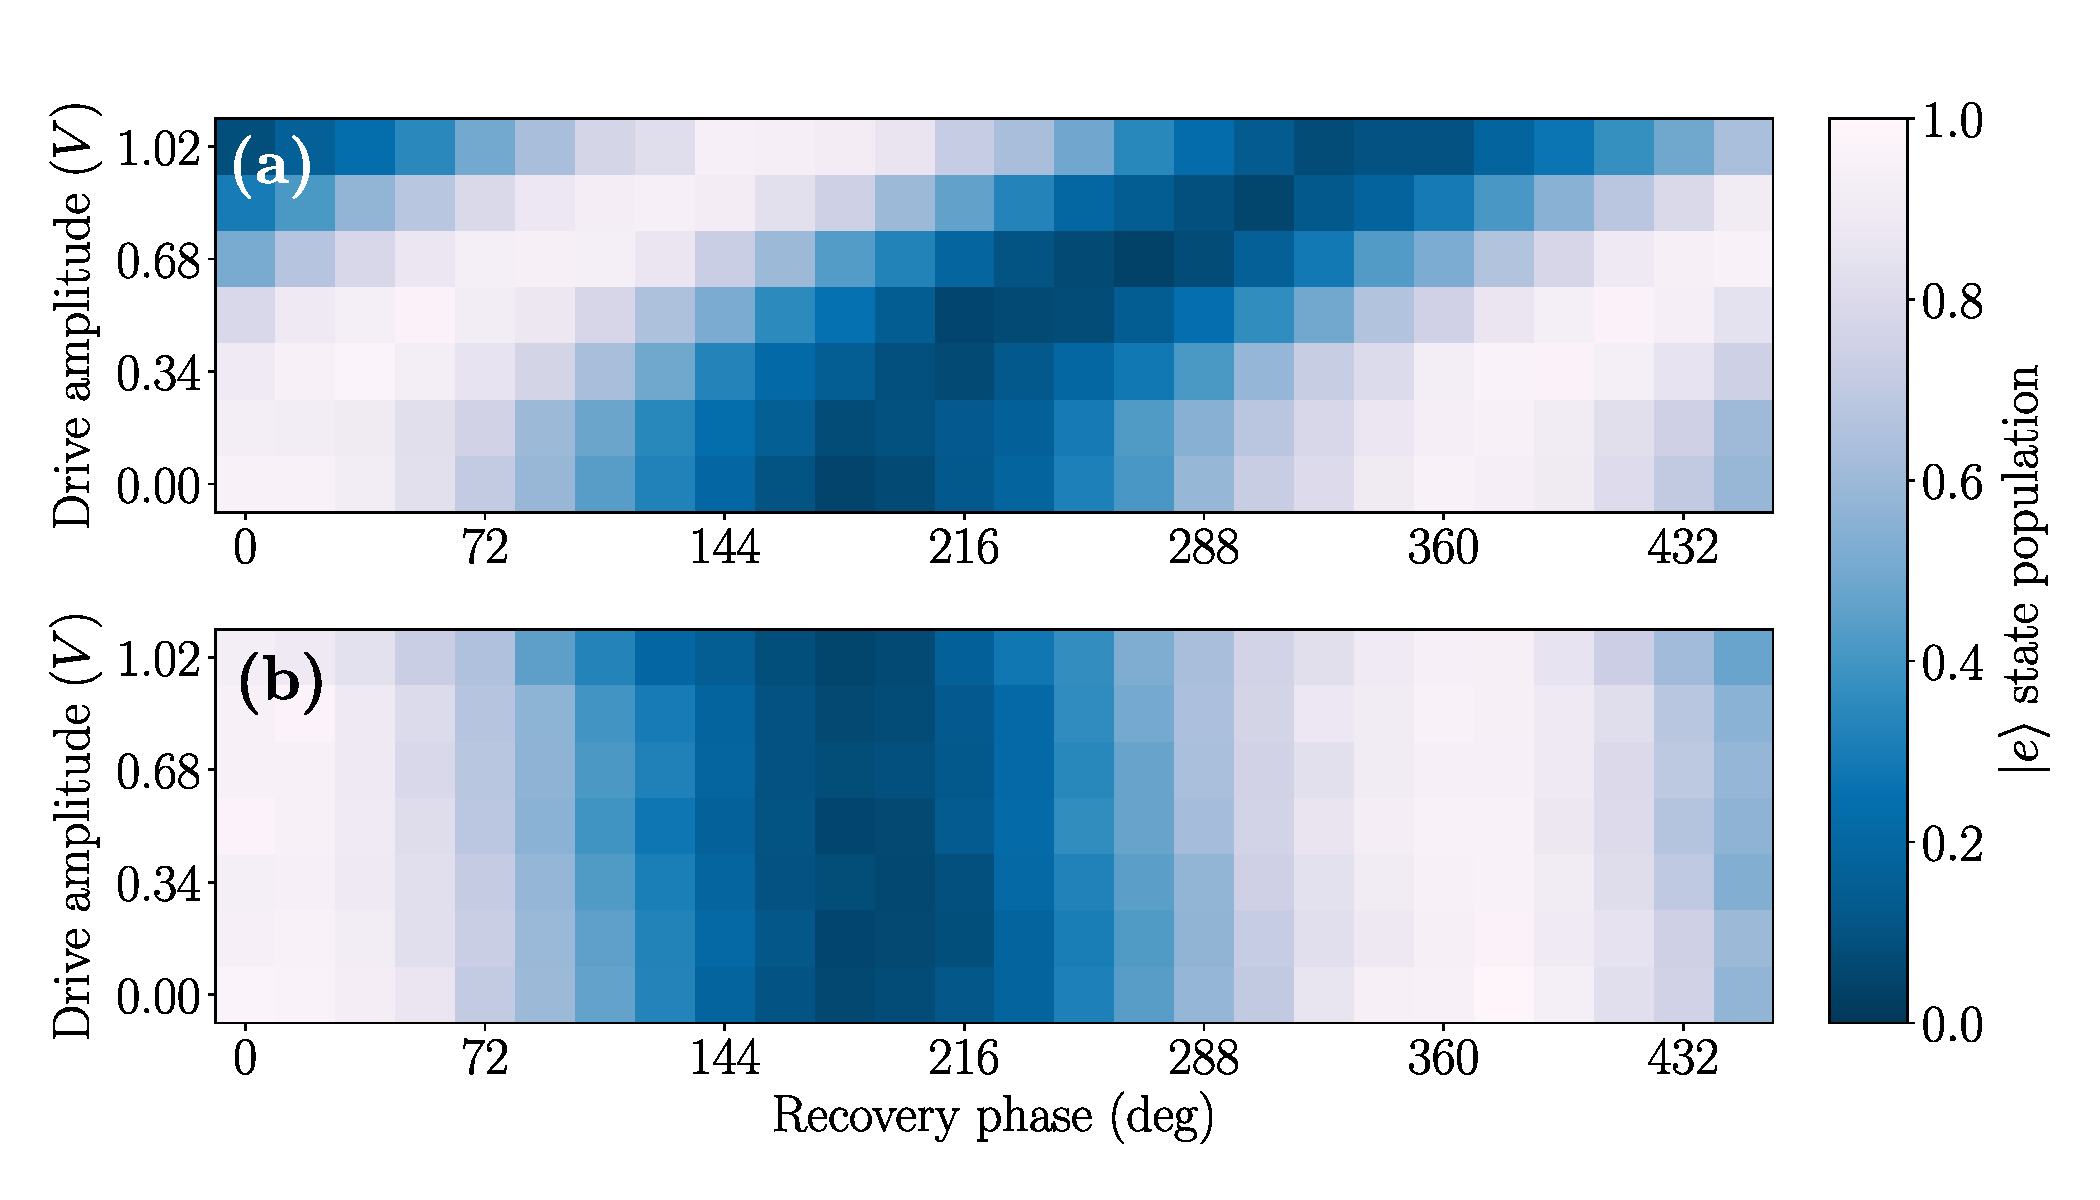
\includegraphics[width=1\linewidth]{Images/Chap2.0/Ramsey_cancellatoin.pdf}
        \label{fig:Ramsey_cancellation}
        \caption{something}
    \end{subfigure}
    \hfill
    \begin{subfigure}[b]{0\textwidth}
        \label{fig:subfig_b}
    \end{subfigure}
    \hfill
    \begin{subfigure}[b]{0\textwidth}
        \label{fig:Ramsey_freq}
    \end{subfigure}
    \vspace{-1cm}
    \caption{Ramsey experiment sweeping recovery pulse's phase $\varphi$ and control drive's amplitude $A$. The results are shown for the run \textbf{(a)} without and \textbf{(b)} with the compensation signal}
    \label{fig:three_subfigures}
\end{figure}
\end{comment}

\begin{figure}
    \centering
    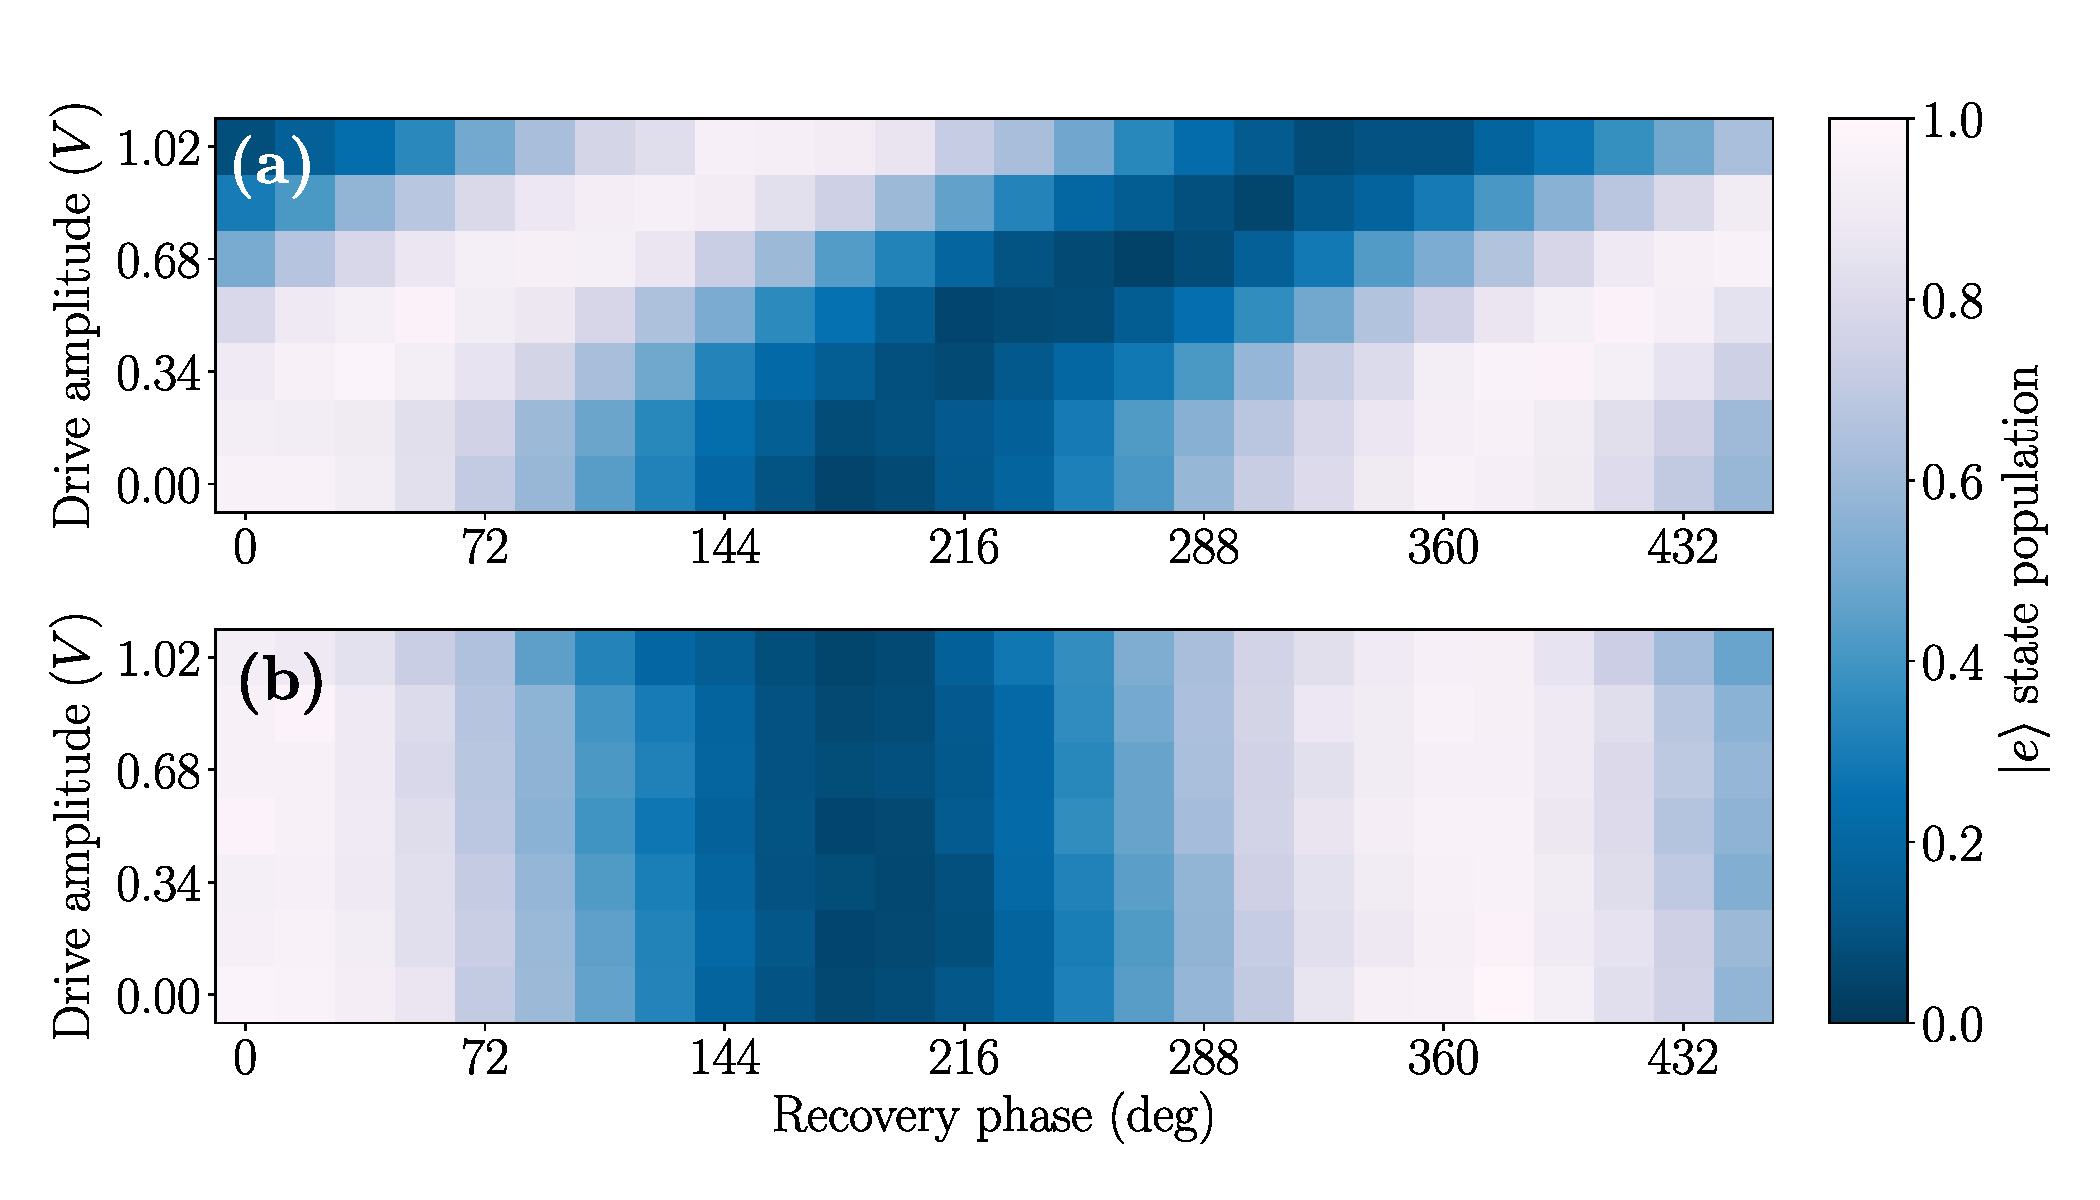
\includegraphics[width=1\linewidth]{Images/Chap2.0/Ramsey_cancellatoin.pdf}
    \vspace{-0.5cm}
    \caption{Ramsey experiment sweeping recovery pulse's phase $\varphi$ and control drive's amplitude $A$. The results are shown for the run \textbf{(a)} without and \textbf{(b)} with the compensation signal. \textbf{(c)}  shows frequency shift due to control drive, as a function of control drive's amplitude, either with or without applying the compensation signal on the target qubit.}
    \label{fig:Ramsey_cancellation}
\end{figure}

By fitting each horizontal line to a cosine wave, we extract the frequency change information encoded in the phase of the cosine wave.
Converting this fitted phase into a frequency as
\begin{equation}
\label{eq:get_frequency}
    \text{frequency} = \frac{\text{phase shift}}{2 \pi \cdot \tau} ,
\end{equation}
reveals the behavior of the target qubit's frequency in relation to the control amplitude.
The outcomes are illustrated in \hyperref[fig:Ramsey_cancellation]{Fig.~\ref{fig:Ramsey_cancellation}c}.
In the absence of compensation parameters, the data follows to a parabolic behaviour, as predicted by \cref{eq:stark_ac}.
However, when the compensation pulse is applied, the extracted frequency shift remains roughly constant.

\begin{comment}
\begin{figure}
    \centering
    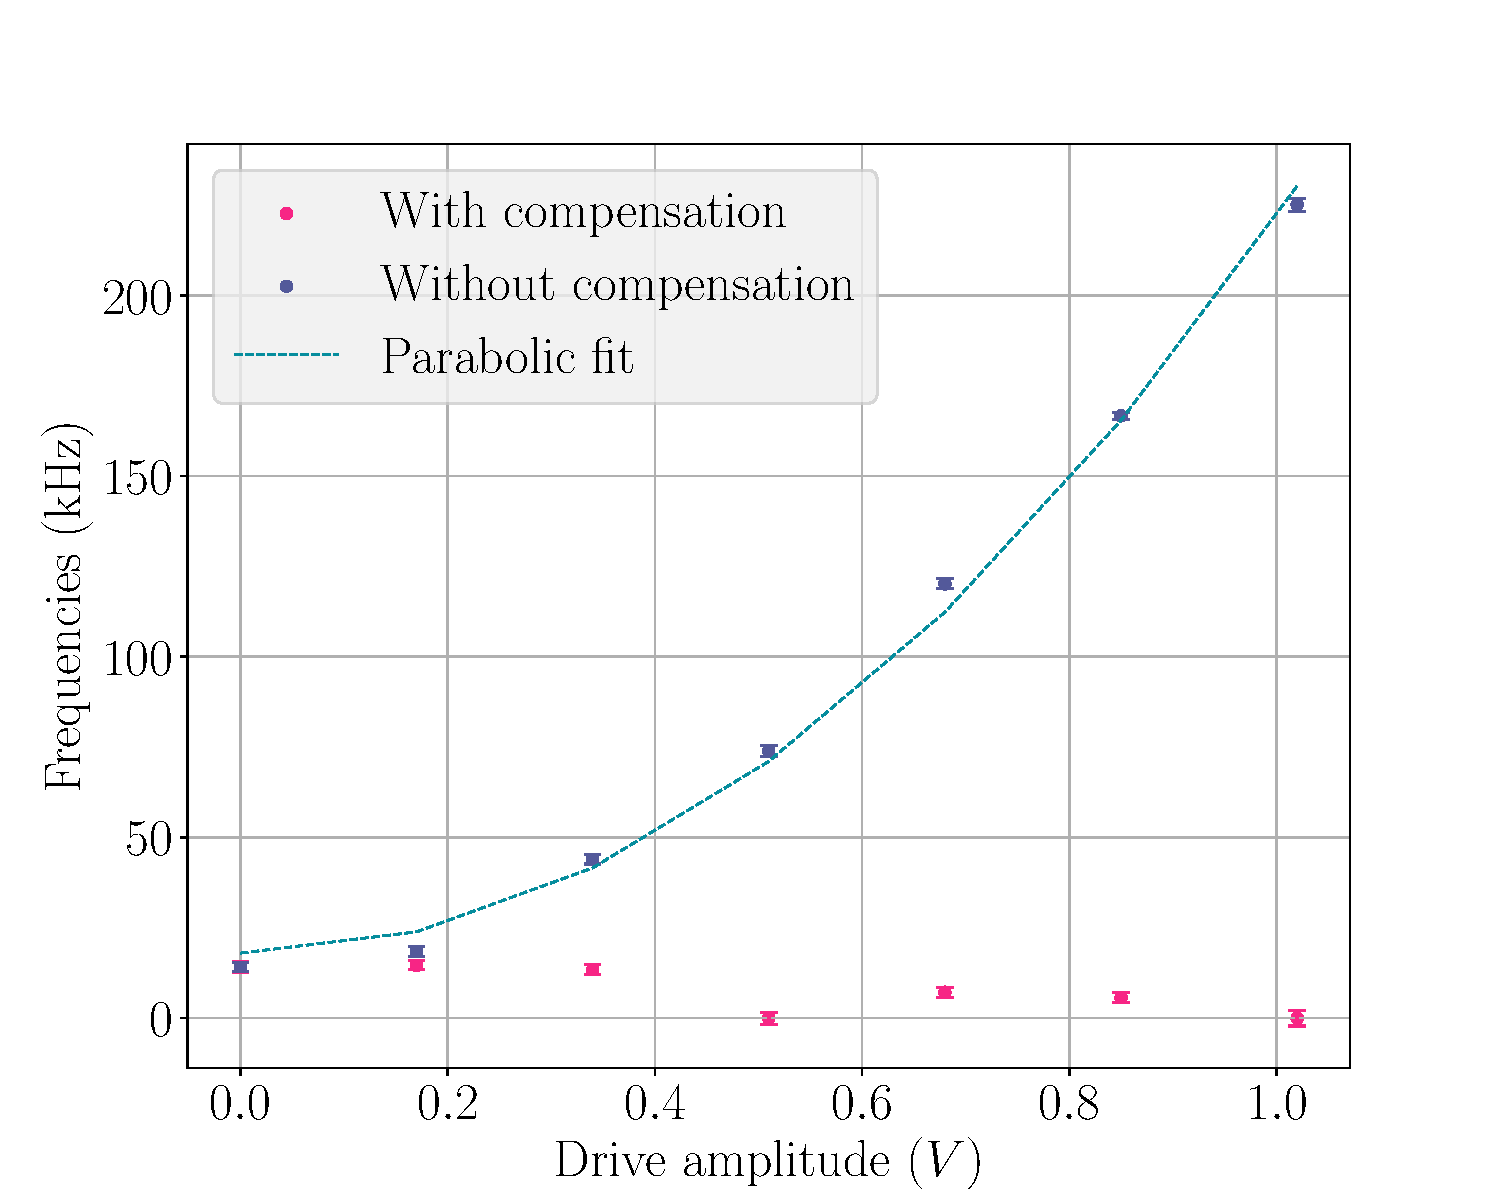
\includegraphics[width=0.75\linewidth]{Images//Chap2.0/frequencies.pdf}
    \caption{Frequency shift due to control drive, as a function of control drive's amplitude, either with or without applying the compensation signal on the target qubit}
    \label{fig:Ramsey_freq}
\end{figure}
\end{comment}

Finally, we confirm the successful cancellation of crosstalk also using a Rabi experiment. 
However, it is known that off-resonant signals induce minimal population changes on the target qubit. 
Furthermore, the compensation parameters we derived strongly rely on the frequency of the control drive.

To test the cancellation with the Rabi experiment, we adjust the frequency of the target qubit to resonate with the control drive. 
Additionally, to mitigate unwanted coupling between the control and target qubits, which are now resonant, we shift the control qubit approximately $\SI{100}{MHz}$ away. 
Subsequently, we collect data with and without the application of the compensation pulse to the target qubit, as a function of the control signal's amplitude and length.
The results of measuring the target qubit after driving the control gate line with a flat-top pulse are depicted in \cref{fig:Rabi_flattop_canc}.

In the absence of the compensation pulse applied to the target qubit, it experiences Rabi oscillations that increase with the control amplitude.
However, these oscillations fail to reach maximum excitation due to imperfect tuning between the control drive's frequency and the target's frequency.

Upon the application of the compensation drive to the target qubit, the control drive ceases to excite the target qubit.
Instead, it is effectively maintained in the ground state.

\begin{figure}
    \centering
    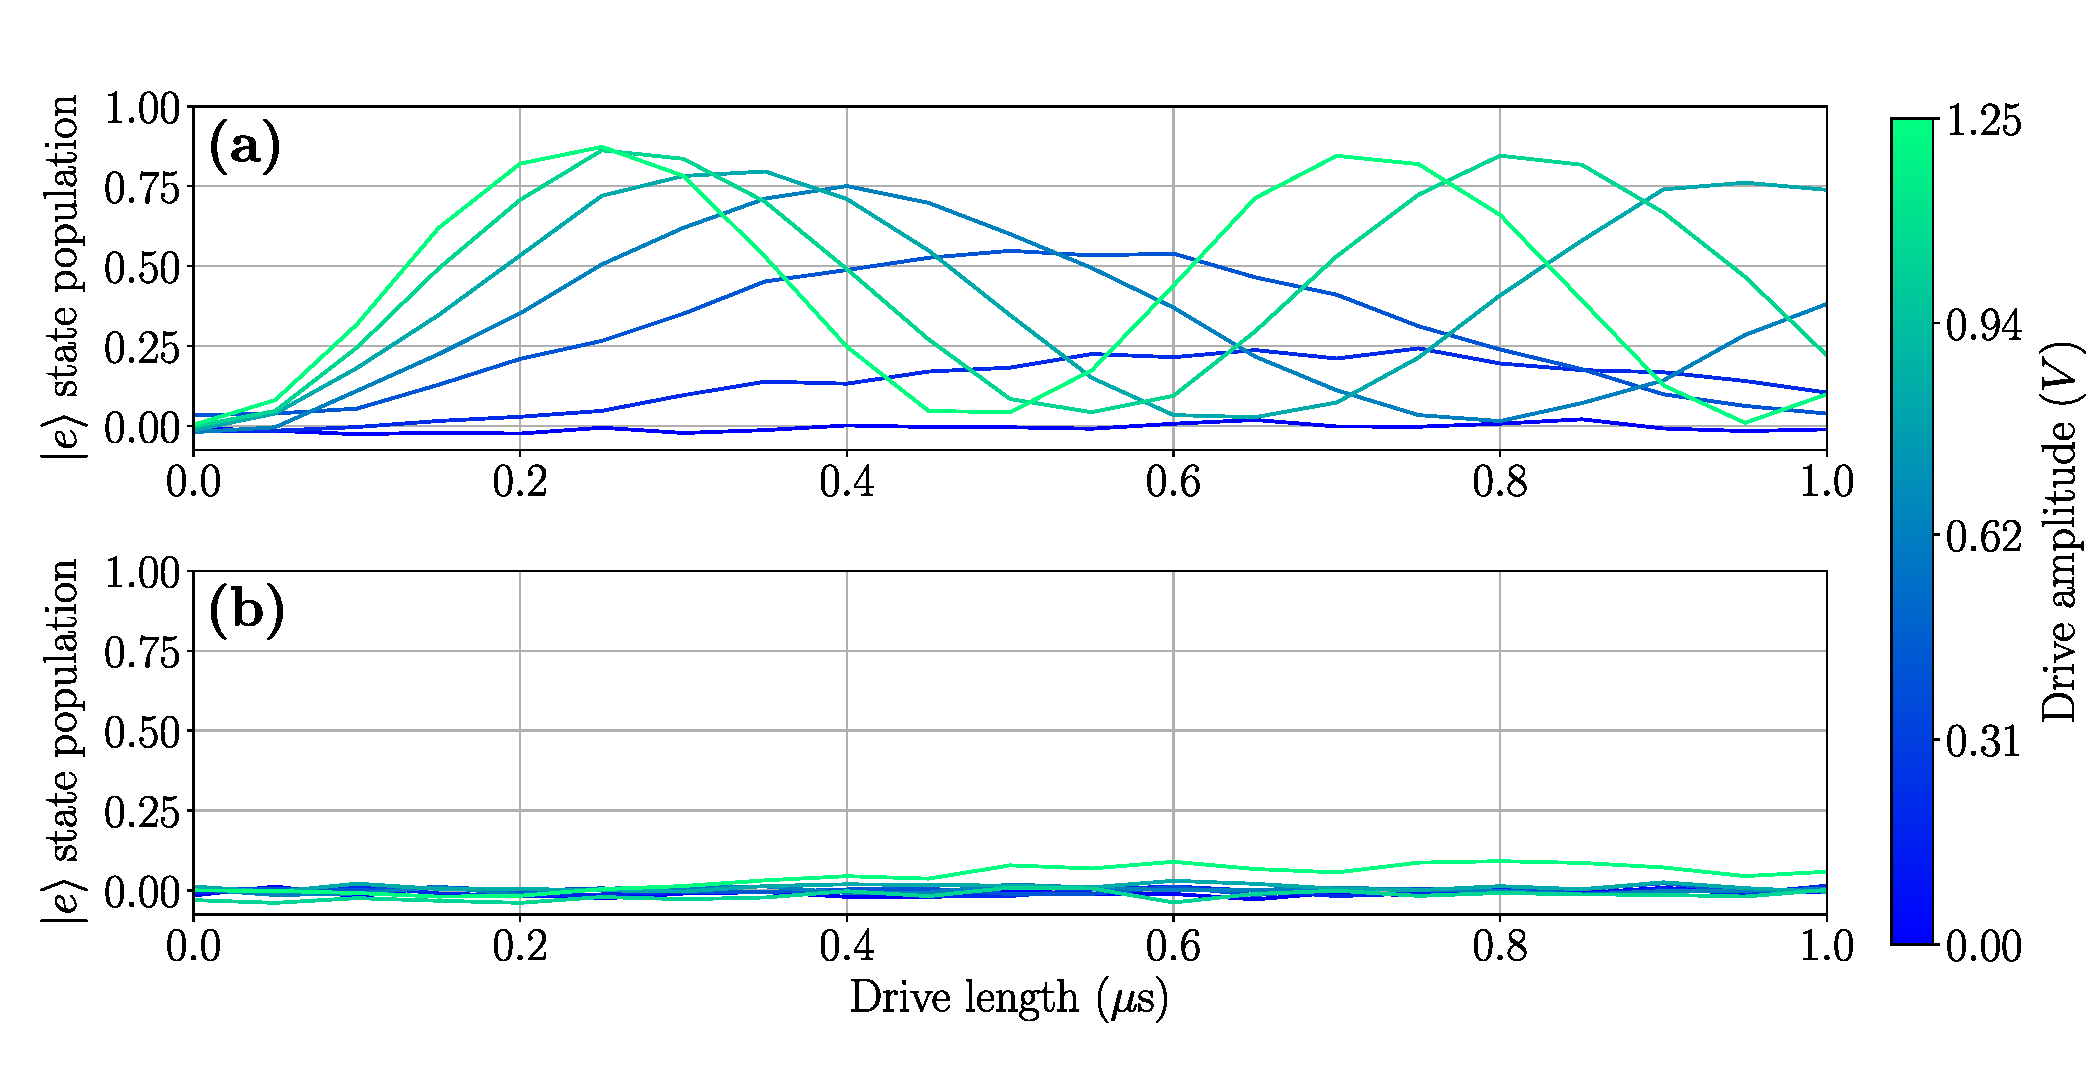
\includegraphics[width=1\linewidth]{Images//Chap2.0/Raby_flattop_cancellation.pdf}
    \vspace{-0.8cm}
    \caption{Population of excited state of the target qubit as a function of the control signal's length, for different control amplitudes, \textbf{(a)} without and \textbf{(b)} with compensation signal}
    \label{fig:Rabi_flattop_canc}
\end{figure}

\section{Measuring with Gaussian-shaped Pulses}
\label{sec:gaussian_shaped}

Ultimately, we iterate through the procedure once more, this time implementing Gaussian-shaped single-qubit pulses.
These pulses are of particular interest to us as they constitute the common single-qubit pulses employed in our protocols.

We perform a gate sequence similar to the previous one to analyze the crosstalk.
However, in this scenario, rather than implementing a prolonged flat-top signal for the control drive, we use multiple Gaussian pulses.
Similarly, we repeat this process for the compensation pulse to ensure it matches the shape and frequency of the control drive. 
In our setup, the Gaussian pulses applied to the control qubit precisely correspond to $\pi$-rotations.
However, as the crosstalk coming from a single $\pi$-pulse on the control qubit is too small, we concatenate 50 $\pi$-pulses together.
A diagram of the gate train employed is depicted in \cref{fig:train_gauss}.

\begin{figure}
    \centering
    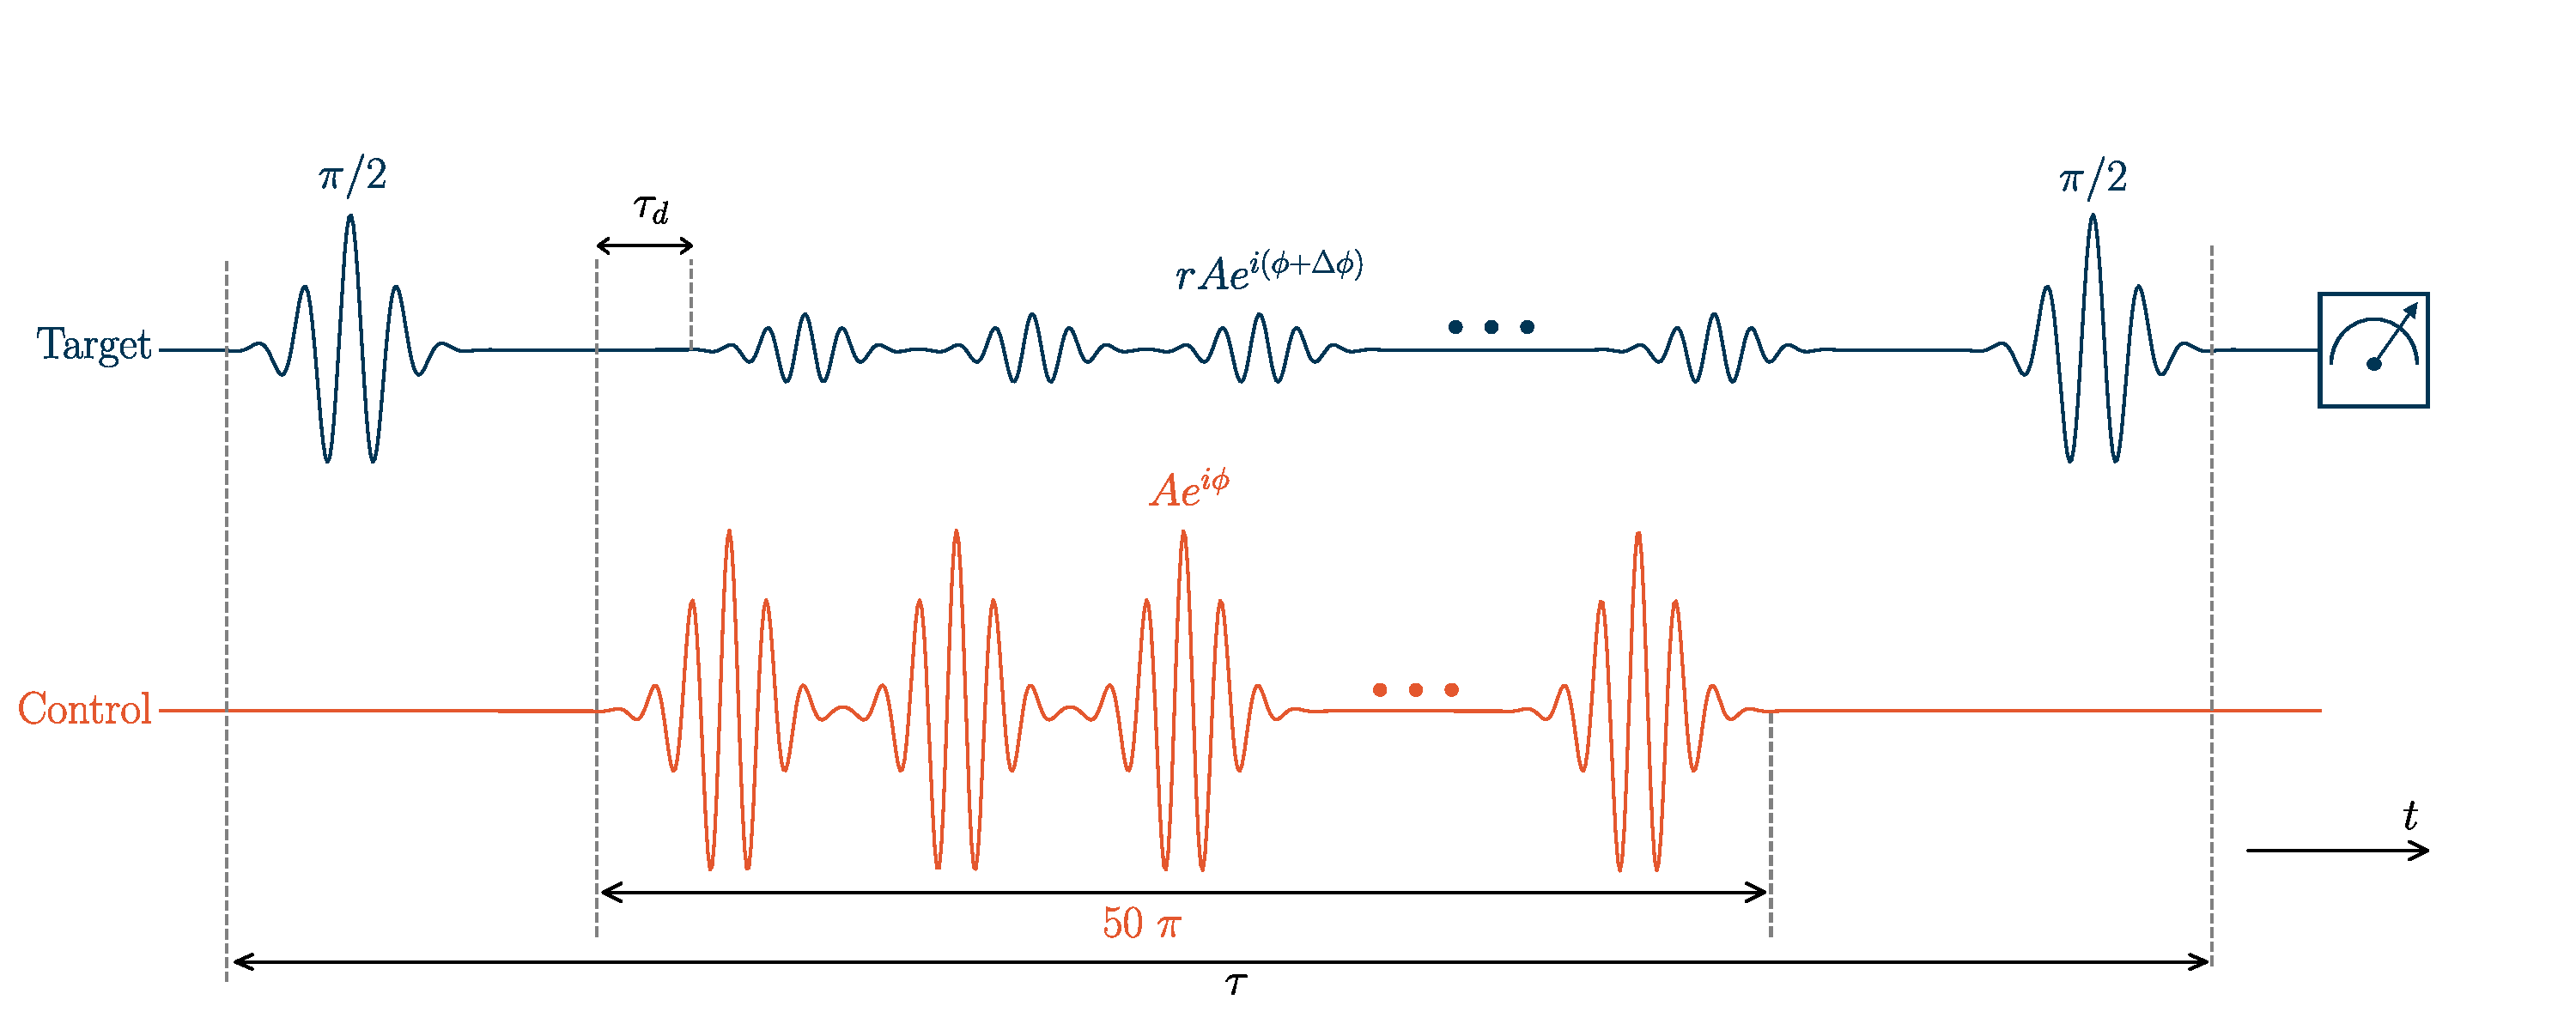
\includegraphics[width=0.95\linewidth]{Images//Chap2.0/diagram_gaussian.pdf}
    \vspace{-0.3cm}
    \caption{Pulse sequence for crosstalk characterization with 50 $\pi$-pulses}
    \label{fig:train_gauss}
\end{figure}

In this scenario, precise synchronization between the control pulse and the compensation pulse becomes important, as they must affect the target qubit simultaneously.
Hence, meticulous calibration of the time delay between these two pulses is crucial.

To align the arrival times of the control drive and the compensation pulse, we simultaneously deliver them to the chip, with the former directed to the control qubit and the latter to the target qubit.
Subsequently, we vary the delay between them.
Lastly, we measure the excited state population of the target qubit.
We expect a sudden transition in the data, attributed to the non-commutativity of rotations around the Bloch sphere.
Subsequent to this, we employ curve fitting using an error function to determine the optimal delay time.
In our configuration, the optimal delay time was determined to be $\tau_d = \SI{-1.41}{ns}$.
The data is shown in \cref{fig:delay}.

\begin{figure}
    \centering
    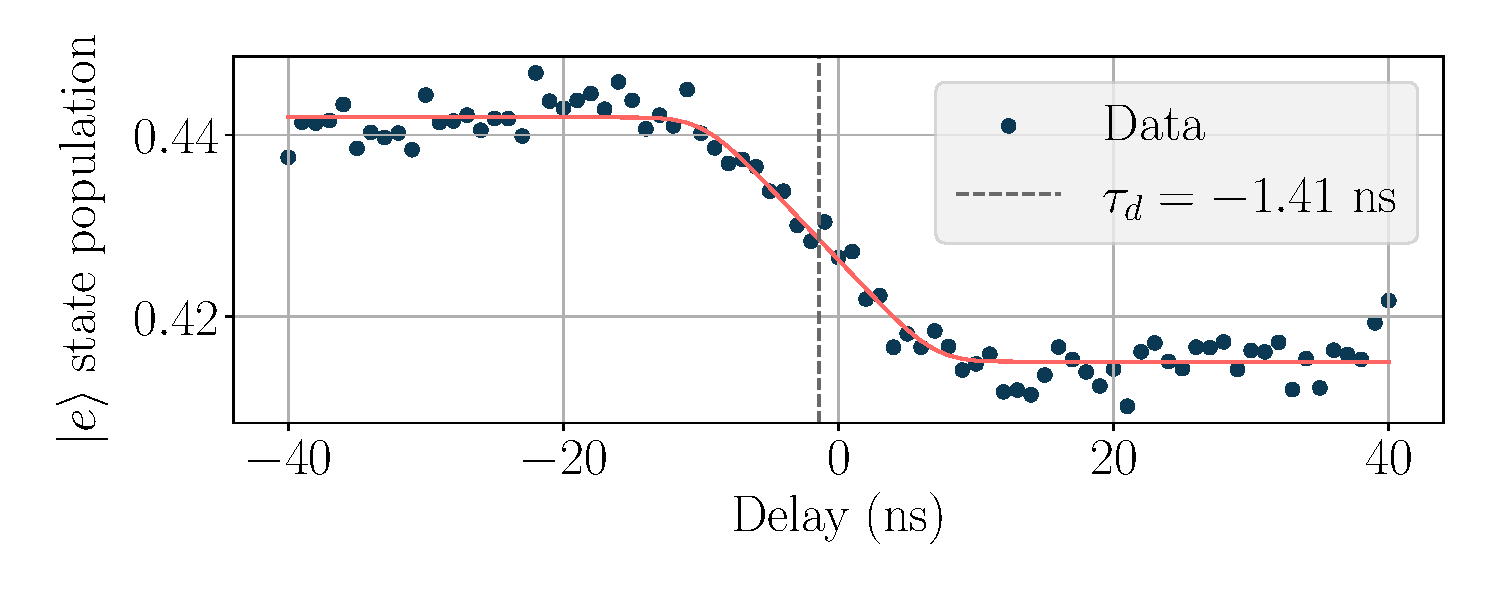
\includegraphics[width=0.8\linewidth]{Images//Chap2.0/delay.pdf}
    \vspace{-0.5cm}
    \caption{Excited state of the target qubit as a function of the delay time between control and compensation pulses. Fit with an error function is shown, together with the optimal delay time found}
    \label{fig:delay}
\end{figure}

% \subsection{Characterization}

The data obtained from measuring the target qubit after implementation of the gate sequence of \cref{fig:train_gauss} is depicted in \cref{fig:circle_pulsed}.
Once more, concentric rings similar to those in the flat-top case are observed.
The red star denotes the center of the rings. 
In this instance, the compensation parameters determined are $r_0 = 0.039$ and $\Delta \phi_0 = 92.6^\circ$.
Notably, the ratio $r$ closely resembles that of the flat-top case, although with a different phase.

The phase-dependant appearance of the rings, appearing oscillating between ground and excited state with respect to the phase of the compensation pulse $\Delta \phi$, presents an intriguing phenomenon.
However, the cause of this discrepancy remains unknown, necessitating further investigation to elucidate its underlying mechanisms.

\begin{comment}
The imperfect appearance of the rings, appearing cut rather than perfectly circular as observed previously, is attributed to the interaction between the two qubits when the control qubit is excited.
In the previous scenario with the flat-top signal, no gates were applied to the control qubit. 
However, in the current setup, we continuously excite and de-excite the control qubit, leading to the observed phenomenon.
\end{comment}

\begin{figure}
    \centering
    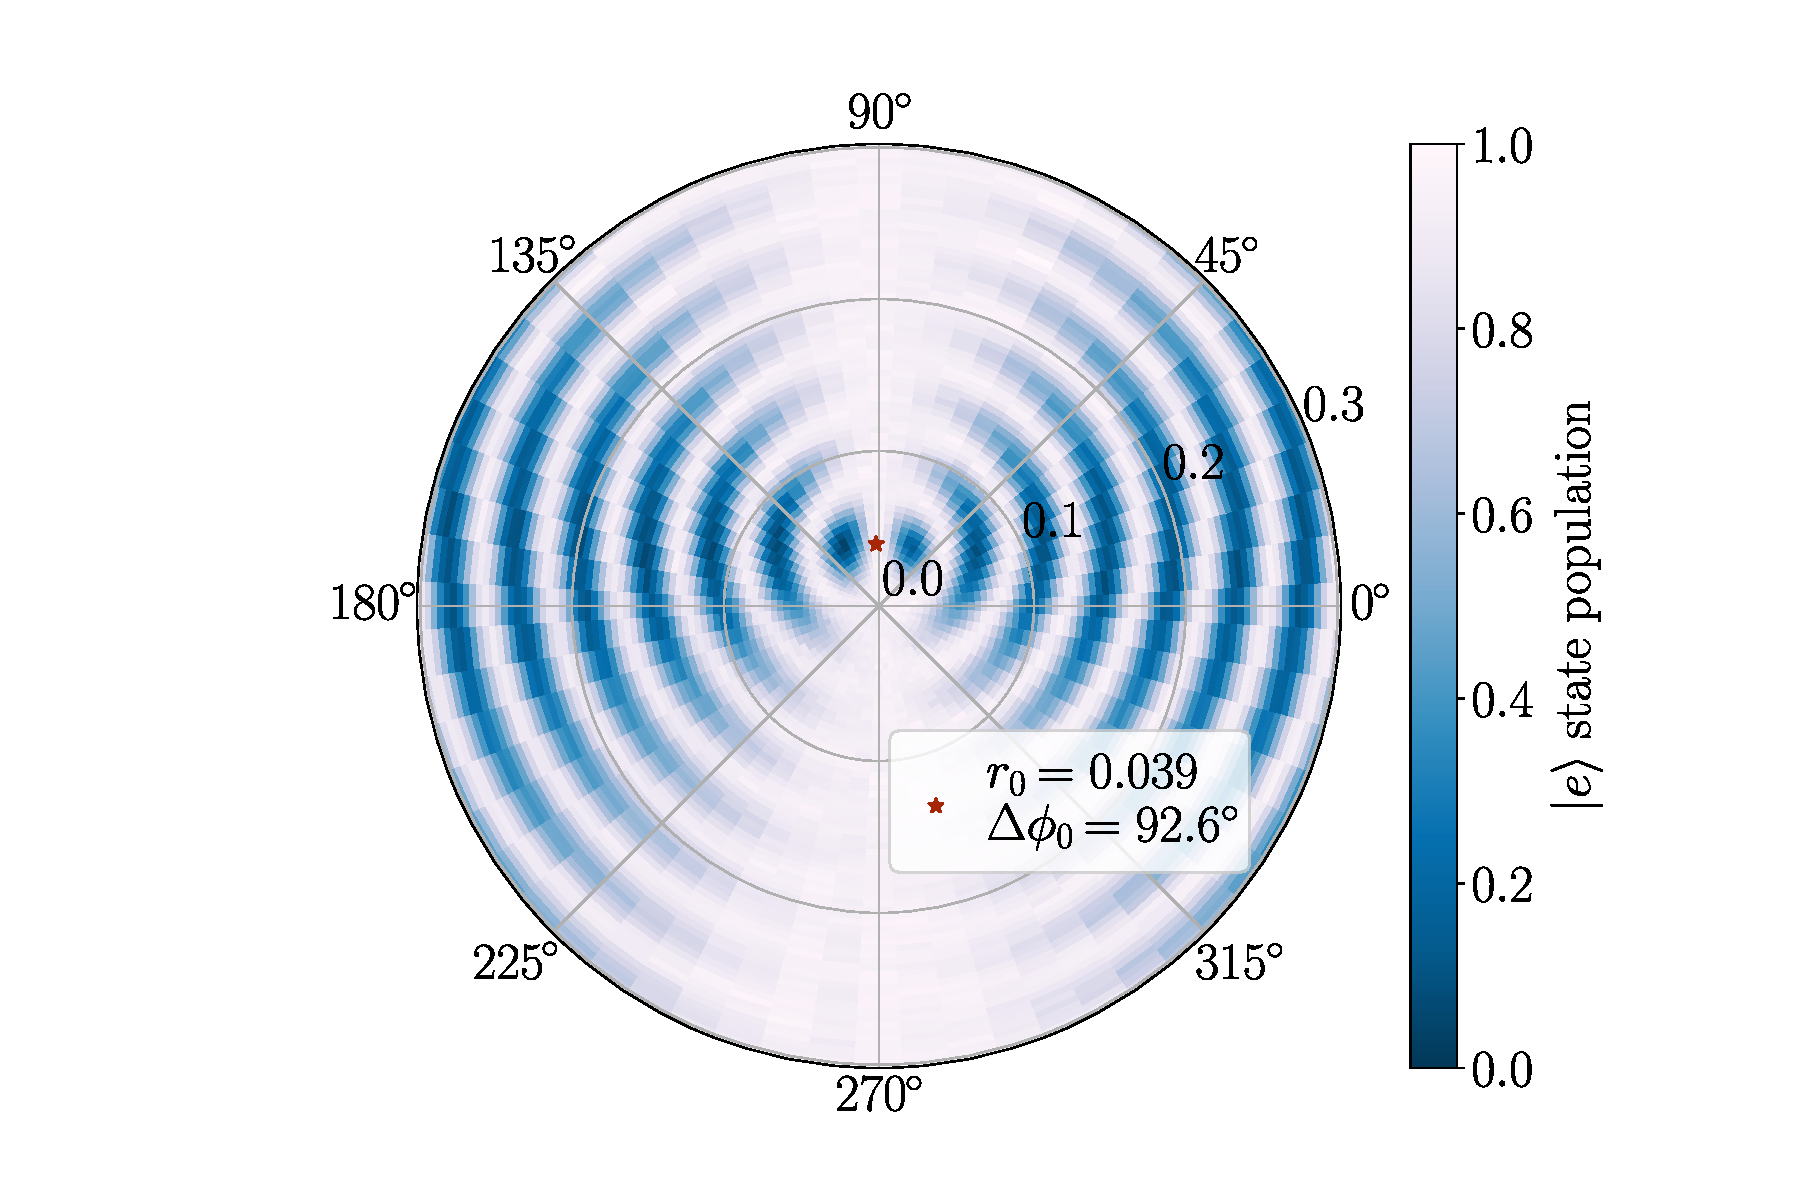
\includegraphics[width=0.8\linewidth]{Images//Chap2.0/circles_pulsed.pdf}
    \vspace{-0.3cm}
    \caption{Excited state of target qubit after gate sequence of  \cref{fig:train_gauss}, as a function of the relative amplitude and phase of compensation pulses. Red star indicates optimal parameters}
    \label{fig:circle_pulsed}
\end{figure}

%\subsection{Cancellation}

\begin{figure}
    \centering
    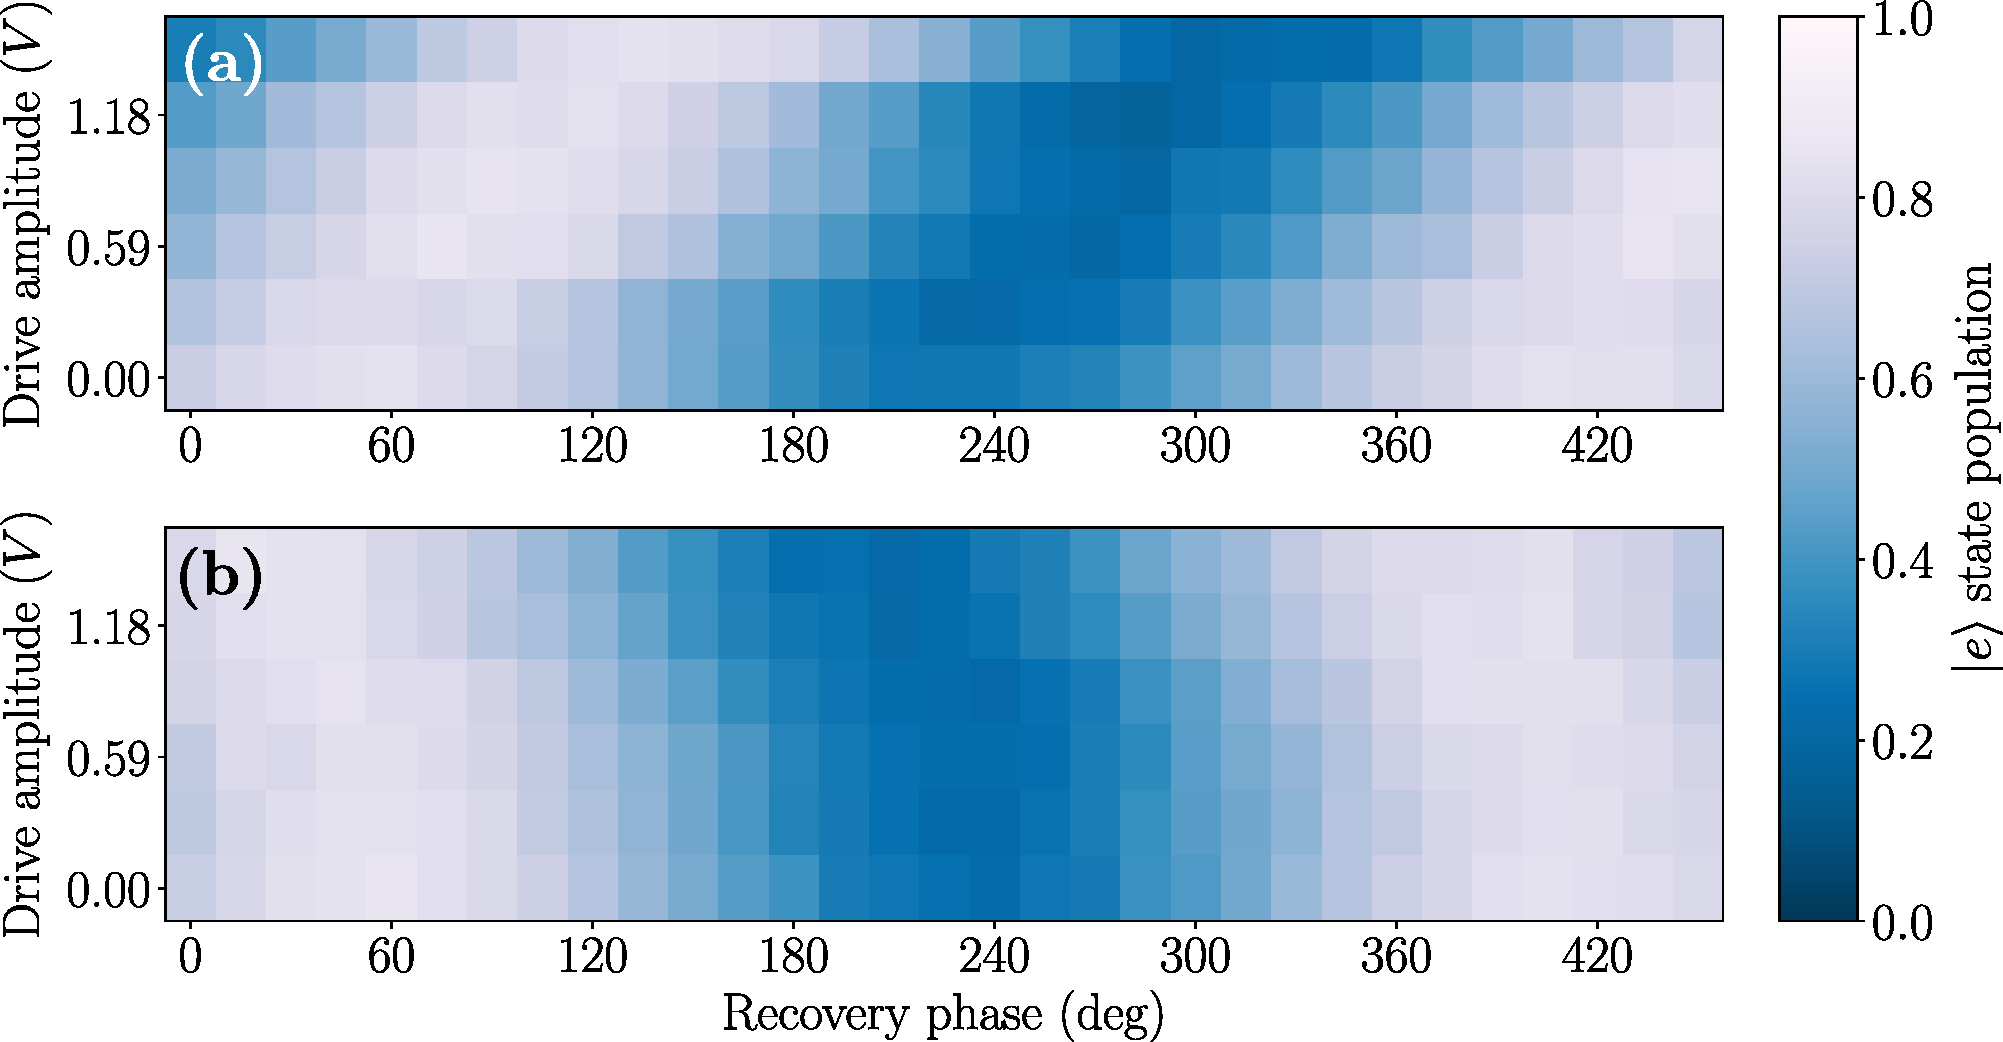
\includegraphics[width=\linewidth]{Images//Chap2.0/Ramsey_cancellatoin_pulsed.pdf}
    \vspace{-0.5cm}
    \caption{Ramsey experiment varying the phase of the recovery pulse $\varphi$ and the amplitude of the control drive $A$. Results are depicted \textbf{(a)} without and \textbf{(b)} with the compensation pulse. \textbf{(c)} shows the frequency shift due to the 200 $\pi$-pulses on the control qubit, as a function of the drive amplitude, both with and without applying the compensation signal.}
    \label{fig:RAMSEY_can_pulsed}
\end{figure}

We validate that the parameters obtained in the pulsed scenario effectively mitigate crosstalk.
Once more, we initiate with a Ramsey measurement.
For this, 200 $\pi$-pulses instead of $50$ were implemented in sequence.
The corresponding dataset is presented in \hyperref[fig:RAMSEY_can_pulsed]{Fig.~\ref{fig:RAMSEY_can_pulsed}a,b}.
In this scenario, it's important to note that while we continue to refer to them as $\pi$-pulses, due to the variation in their amplitude, they no longer precisely correspond to $\pi$-pulses on the control qubit.

\begin{comment}
\begin{figure}[t!]
    \centering
    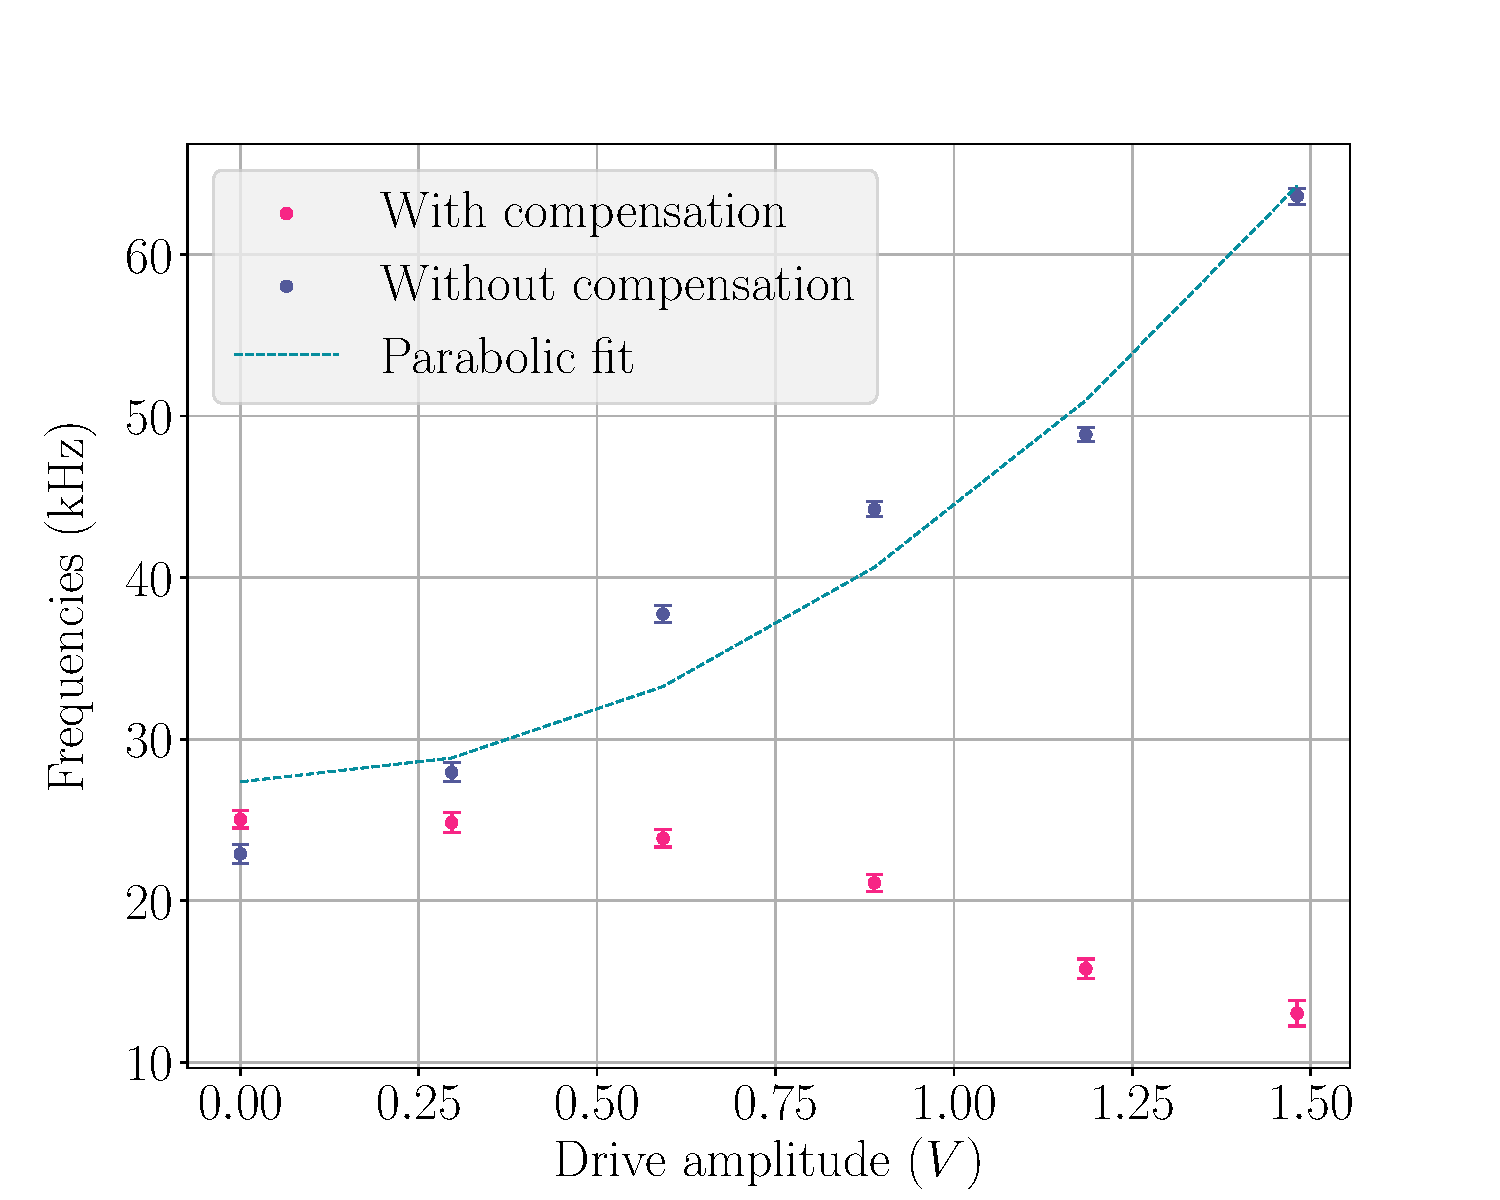
\includegraphics[width=0.75\linewidth]{Images//Chap2.0/frequencies_200.pdf}
    \caption{Frequency shift due to the 200 $\pi$-pulses on the control qubit, as a function of the drive amplitude, both with and without applying the compensation signal}
    \label{fig:Freq_pulsed}
\end{figure}
\end{comment}

A similar analysis is performed on the dataset, involving fitting the data with a cosine wave for each driving amplitude to calculate the frequency shift once more using \cref{eq:get_frequency}.
The outcomes of this analysis are illustrated in \hyperref[fig:RAMSEY_can_pulsed]{Fig.~\ref{fig:RAMSEY_can_pulsed}c}.

On this occasion, the observed cancellation appears to be imperfect.
Our hypothesis suggests that this may be attributed to the shorter duration of the pulses, resulting in a broader bandwidth in Fourier space.
Consequently, compensating for all frequency components simultaneously becomes a more challenging task. 
Nevertheless, despite these challenges, the discernible reduction in the AC Stark effect remains evident.

Finally, we verify the successful cancellation of the crosstalk effect through a Rabi experiment.
Once again, we move the target qubit to be resonant with the drive while simultaneously shifting the control qubit away of at least $\SI{100}{MHz}$.
The population data of the excited state $\ket{e}$ for the target qubit is presented as a function of the drive amplitude in \cref{fig:Rabi_canc_pulsed}.
We clearly observe how, in this instance as well, the crosstalk effect is effectively neutralized using our method.

Our interpretation of the “beating" pattern observed in the plot depicted in \cref{fig:Rabi_canc_pulsed} is as follows: applying the control drive induces Rabi oscillations on the target qubit.
However, the control drive is switched off before the target qubit can fully reach the excited state.
Consequently, the target qubit experiences multiple rapid not-complete Rabi oscillations, leading to the observed beating pattern in the plot.
%causes the target qubit frequency to lag behind the induced AC Stark frequency.
%This temporal non-adiabaticity results in the generation of the observed beating pattern.

The observed dependencies of the rings in \cref{fig:circle_pulsed} on the phase of the compensation pulse $\Delta \phi$ may be attributed to the non-adiabatic effect or the broader bandwidth of the pulses in Fourier space. 
Additionally, the incomplete cancellation of the ZZ interaction between the qubits could also contribute to this phenomenon.
However, despite these hypotheses, a definitive model and explanation for the observed data pattern have yet to be established.

\begin{figure}
    \centering
    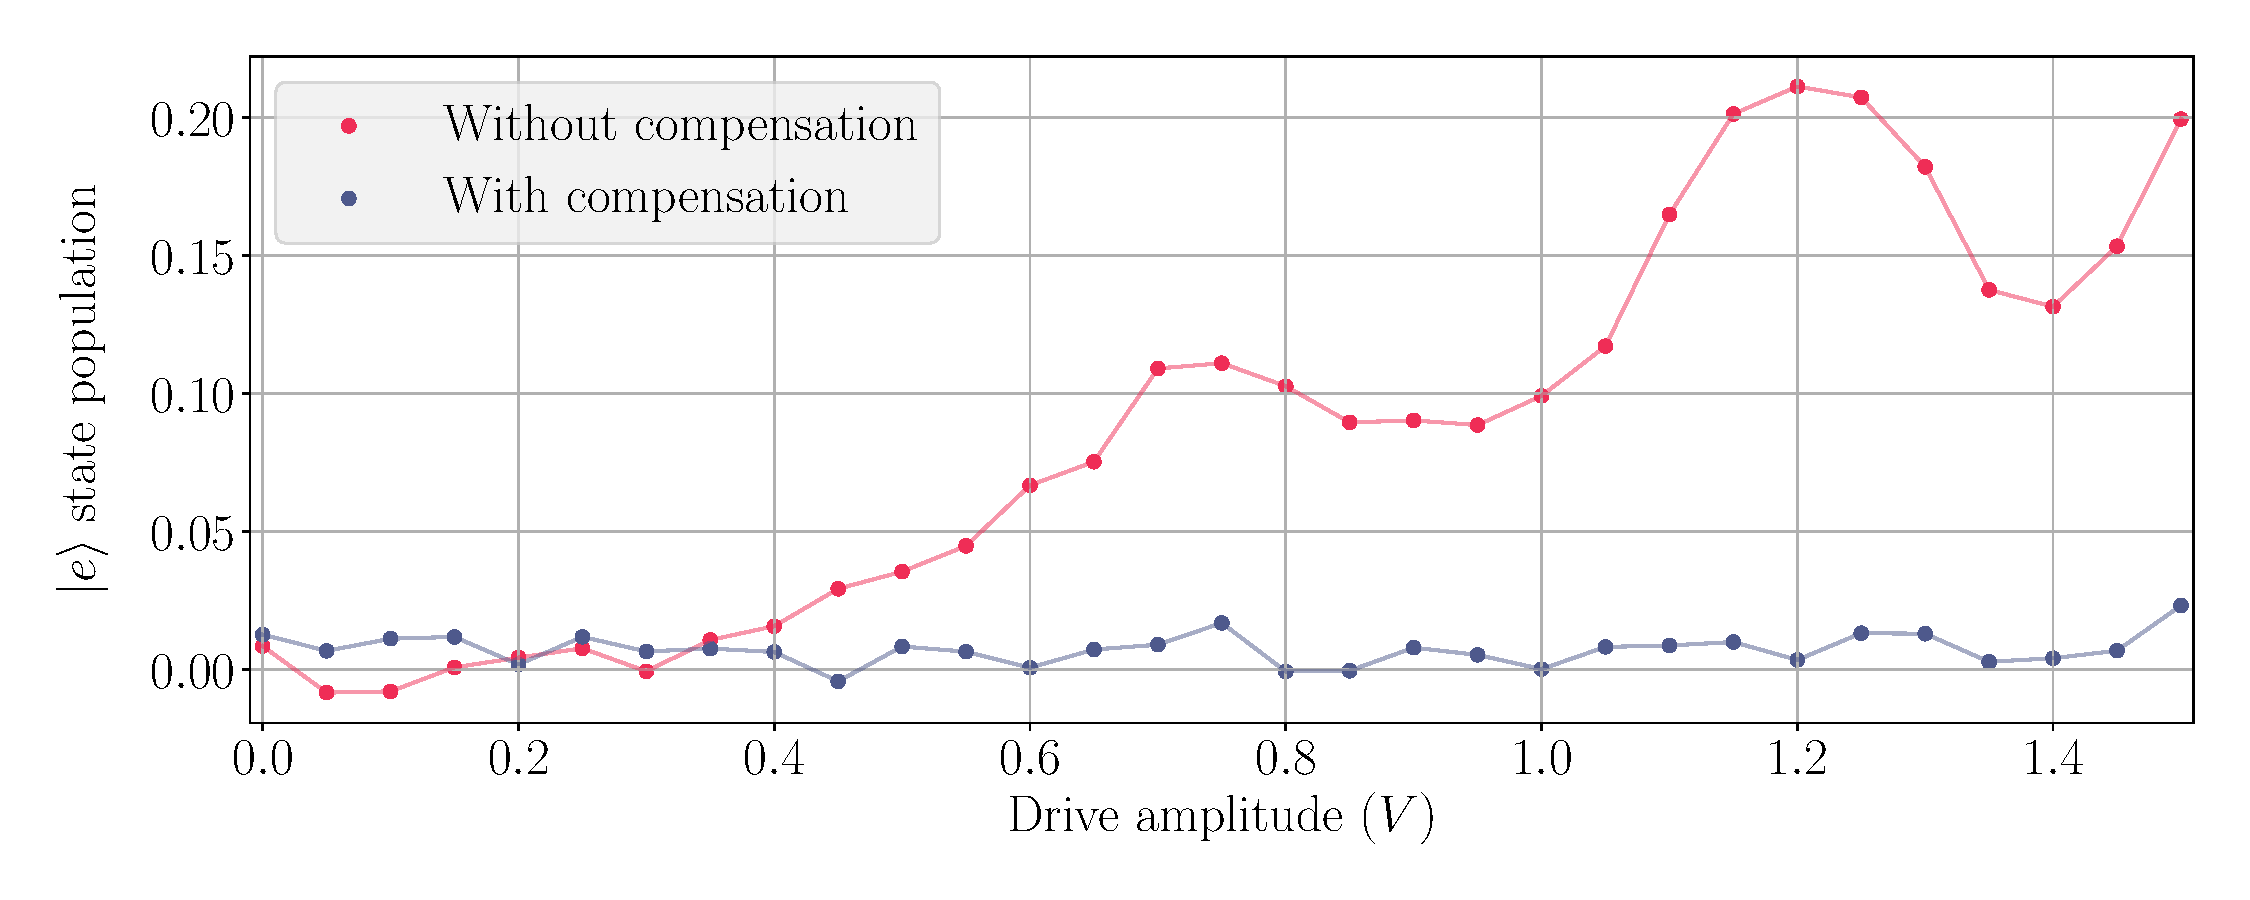
\includegraphics[width=0.75\linewidth]{Images//Chap2.0/Rabi_pulsed_cancellation.pdf}
    \caption{$\ket{e}$ population of target qubit as a function of the drive amplitude, both with and without compensation pulses}
    \label{fig:Rabi_canc_pulsed}
\end{figure}